\documentclass[a4paper]{article}

% Basic packages
\usepackage{fontspec}
\XeTeXlinebreaklocale "zh"    % 启用中文断行（XeTeX 内建，无需 xeCJK）
\XeTeXlinebreakskip = 0pt plus 1pt
\setmainfont{Songti SC}
\setsansfont{Heiti SC}
\setmonofont{Menlo}
\usepackage{amsmath, amssymb}
\usepackage{graphicx}
\usepackage[margin=2.5cm]{geometry}
\usepackage[most]{tcolorbox}
\usepackage{etoolbox}
\usepackage{listings}
\usepackage{hyperref}
\usepackage{booktabs}
\usepackage{subcaption}
\usepackage{float}

% Chinese font setup (macOS system fonts, no ctex needed)
\setmainfont{Songti SC}
\setsansfont{Heiti SC}
\setmonofont{Menlo}
\newcommand{\song}{\fontspec{Songti SC}}
\newcommand{\hei}{\fontspec{Heiti SC}}
\newcommand{\kai}{\fontspec{KaiTi}}
\newcommand{\fangsong}{\fontspec{FangSong}}

% ===== Highlight boxes =====
\newtcolorbox{knowledgebox}[1]{
    enhanced, colback=blue!5!white, colframe=blue!75!black, colbacktitle=blue!75!black,
    coltitle=white, fonttitle=\bfseries, title=#1, attach boxed title to top left={yshift=-2mm, xshift=2mm},
    boxrule=1pt, sharp corners
}

\newtcolorbox{importantbox}[1]{
    enhanced, colback=yellow!10!white, colframe=yellow!80!black, colbacktitle=yellow!80!black,
    coltitle=black, fonttitle=\bfseries, title=#1, sharp corners
}

\newtcolorbox{warningbox}[1]{
    enhanced, colback=red!5!white, colframe=red!75!black, colbacktitle=red!75!black,
    coltitle=white, fonttitle=\bfseries, title=#1, sharp corners
}

\newtcolorbox{practicebox}[1]{
    enhanced, colback=green!5!white, colframe=green!60!black, colbacktitle=green!60!black,
    coltitle=white, fonttitle=\bfseries, title=#1, sharp corners
}

% ===== Code listings =====
\lstset{
    basicstyle=\ttfamily\small,
    keywordstyle=\color{blue},
    stringstyle=\color{red!60!black},
    commentstyle=\color{green!60!black},
    breaklines=true,
    frame=single,
    numbers=left,
    numberstyle=\tiny\color{gray},
    captionpos=b,
    extendedchars=false
}

% ===== Front-page metadata =====
\newcommand{\notetitle}{CS336 Lecture 6：GPU Kernels 与 Triton}
\newcommand{\notesubtitle}{Stanford CS336: Language Modeling from Scratch (Spring 2025)}
\newcommand{\noteauthors}{讲师：Percy Liang \quad 笔记：ZCode}
\newcommand{\notedate}{2026-07-14}
\newcommand{\videochannel}{Stanford CS336}
\newcommand{\videopublishdate}{2025 Spring}
\newcommand{\videoduration}{80 分钟}
\newcommand{\videourl}{https://www.youtube.com/watch?v=E8Mju53VB00}
\newcommand{\videocoverpath}{cover.jpg}

\begin{document}

% ===== Title page =====
\begin{titlepage}
\centering
{\Large 课程笔记\par}
\vspace{1.2cm}
{\huge\bfseries \notetitle\par}
\vspace{0.3cm}
{\large \notesubtitle\par}
\vspace{0.5cm}
{\large \noteauthors\par}
\vspace{0.3cm}
{\large \notedate\par}
\vspace{1.0cm}

\includegraphics[width=0.82\textwidth,height=0.40\textheight,keepaspectratio]{\videocoverpath}\par

\vfill
\begin{tcolorbox}[width=0.9\textwidth, colback=black!2!white, colframe=black!60, sharp corners]
\textbf{视频作者/频道}：\videochannel\par
\textbf{发布日期}：\videopublishdate\par
\textbf{视频时长}：\videoduration\par
\textbf{视频链接}：\href{\videourl}{\nolinkurl{\videourl}}
\end{tcolorbox}
\end{titlepage}

\tableofcontents
\newpage

%% --- 正文内容开始 ---

\section{导论：为 GPU 写高性能代码}

本讲的主题是\textbf{如何为 GPU 编写高性能代码}。这是 Assignment 2 的直接前置知识——在作业里你将不得不做大量 profiling、亲手写一个 FlashAttention 2 的 Triton kernel，并让所有这些组件跑得足够快。本讲会一路钻到底，从最上层的 Python 计时，下钻到 NVIDIA 的 Nsight Systems profiler，再下钻到几乎贴近机器码的 PTX 汇编，搞清楚 GPU 到底在干什么。

\begin{knowledgebox}{本讲的整体路线图}
\begin{enumerate}
    \item \textbf{GPU 回顾}：SM、thread block、warp、内存层级、算术强度。
    \item \textbf{Benchmarking（基准测试）}：如何正确测量 wall-clock 时间——warm-up、CUDA synchronize、重复取平均。
    \item \textbf{Profiling（性能剖析）}：用 \texttt{torch.profiler} 和 NVIDIA Nsight Systems 看进函数内部、看 CPU/GPU 异步执行。
    \item \textbf{Kernel fusion（算子融合）}：为什么把多个小 kernel 融合成一个大 kernel 会快得多。
    \item \textbf{GELU 的四种写法}：naive PyTorch → 手写 CUDA → Triton → \texttt{torch.compile}，逐一 benchmark 对比。
    \item \textbf{Triton softmax}：一个需要做 reduction 的非平凡 kernel 示例。
\end{enumerate}
\end{knowledgebox}

\section{GPU 执行模型回顾}

\subsection{SM、线程块与内存层级}

\begin{figure}[H]
\centering
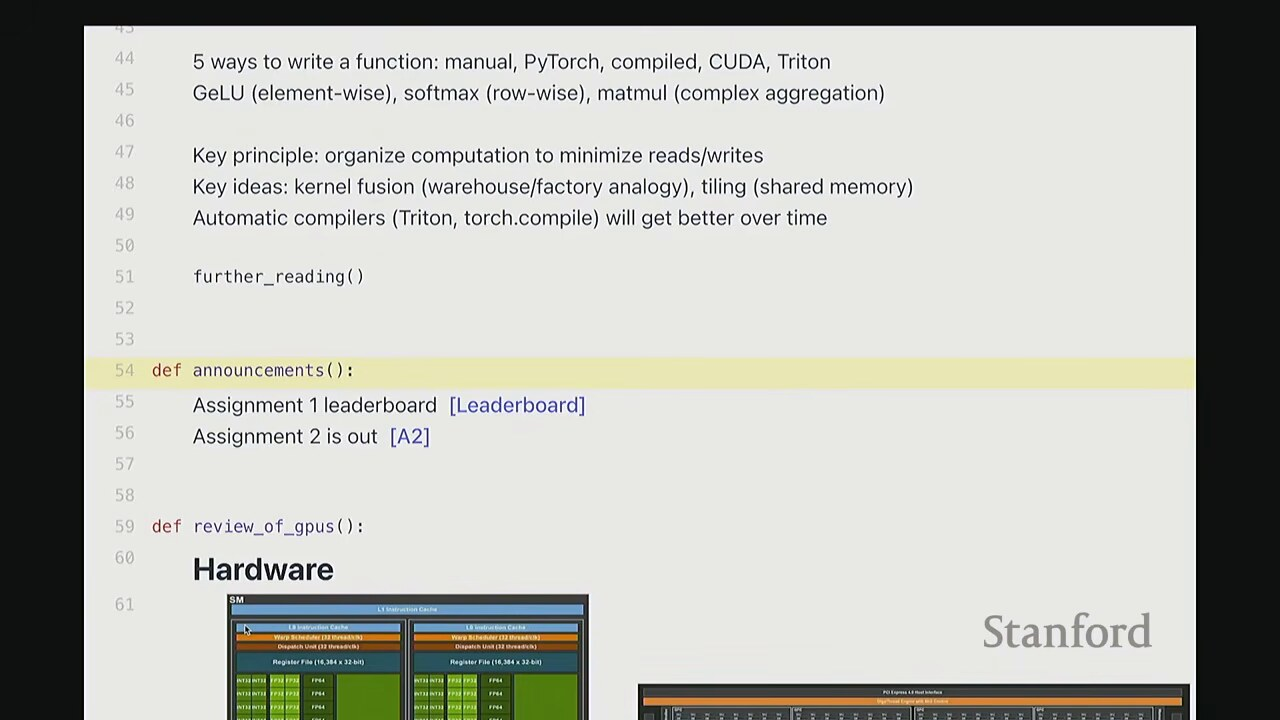
\includegraphics[width=\textwidth]{figures/fig_01_gpu_arch.jpg}
\caption{GPU 硬件回顾：streaming multiprocessor (SM)、thread block 与内存层级（DRAM / cache / register file）\protect\footnotemark}
\end{figure}
\footnotetext{视频画面时间区间：00:02:00--00:02:15。}

当我们面对一片 A100 或 H100 时，它内部有大量\textbf{streaming multiprocessor（SM，流式多处理器）}。每个 SM 内部有大量计算单元（INT32、FP32 等），并会发射出大量\textbf{线程（thread）}。围绕这些计算单元有一套\textbf{内存层级}：

\begin{itemize}
    \item \textbf{DRAM / global memory}：容量大、速度慢，所有 SM 共享。
    \item \textbf{L1/L2 cache}：比 DRAM 快得多。
    \item \textbf{register file（寄存器堆）}：极其快，每个线程本地访问。本讲会反复用到寄存器。
    \item \textbf{shared memory}：位于 SM 内部、近似 L1 速度，供同一 thread block 内的线程通信。
\end{itemize}

\begin{figure}[H]
\centering
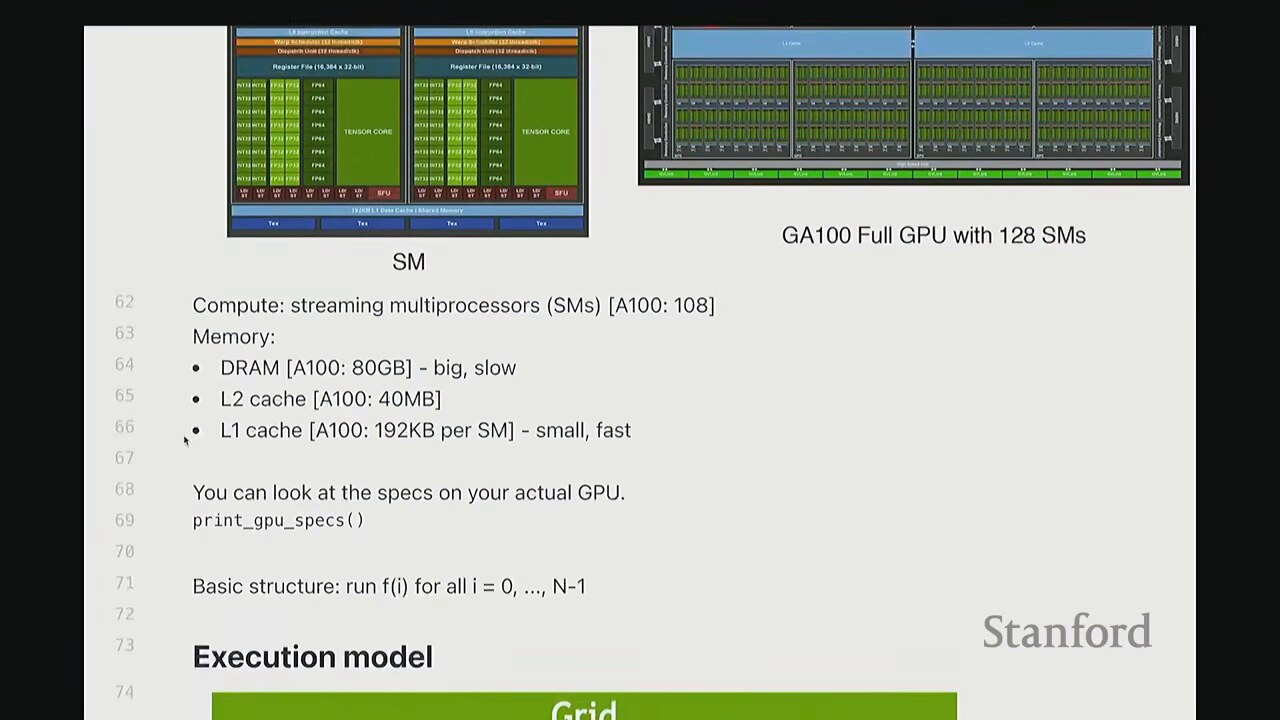
\includegraphics[width=\textwidth]{figures/fig_02_thread_blocks.jpg}
\caption{Thread block 调度：一个 block 整体落在单个 SM 上，block 内通过 shared memory 通信\protect\footnotemark}
\end{figure}
\footnotetext{视频画面时间区间：00:03:00--00:03:15。}

执行模型的基本单位是\textbf{thread block（线程块）}：一个 block 会被调度到\emph{单个 SM} 上执行，这是我们在写 Triton 时要思考的"原子单位"。block 内部的线程才是真正做计算的。为什么要有 block 这个概念而不是让所有线程平等地共享一个大全局？因为 block 内部可以通过\textbf{shared memory} 做线程间通信（速度近似 L1），而跨 block 通信则极其昂贵——所以任何需要线程协作的数据（比如矩阵乘里要传递的中间结果），都应尽量留在同一个 block / 同一个 SM 内。

\subsection{Warp 与 Wave：调度粒度}

\begin{figure}[H]
\centering
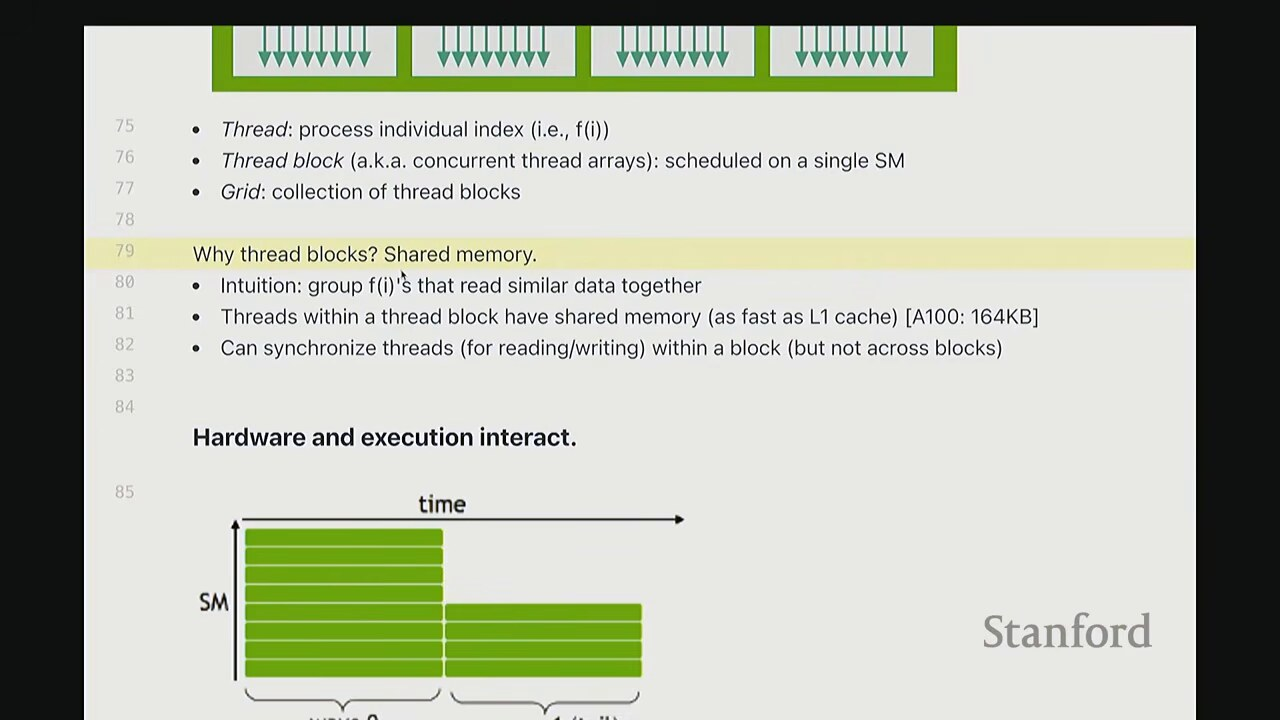
\includegraphics[width=\textwidth]{figures/fig_03_waves_warp.jpg}
\caption{Warp（32 线程一组）与 wave（跨 SM 的调度波）：wave quantization 会影响利用率\protect\footnotemark}
\end{figure}
\footnotetext{视频画面时间区间：00:04:00--00:04:15。}

\textbf{Warp（线程束）}是 32 个连续线程构成的一组，SM 上以 warp 为单位一起发射执行。warp 存在的意义是\emph{减少控制电路}：既然 32 个线程同时执行，就不必为每个线程单独配一套控制/分支预测逻辑，只需为每 32 个线程配一个 warp scheduler。这正是 GPU 与 CPU 的核心 trade-off——CPU 把大量晶体管花在控制、分支预测上；GPU 则把面积尽量留给计算，控制更简单。

\textbf{Wave（波）}是另一个对性能重要但平时不太显眼的概念：当 thread block 数量超过 SM 数量时，硬件会把 block 分批，每一批称为一个 wave。我们希望让所有 wave 工作量相等——理想情况下 thread block 数量是 SM 数量的整数倍，并且远大于 SM 数量，以避免\textbf{wave quantization}（最后一批只有零星几个 block 在跑，造成尾部利用率塌陷）。

\begin{importantbox}{一句话总结 GPU 编程的两个目标}
\begin{enumerate}
    \item \textbf{让 SM 都忙起来}：thread block 数量 $\gg$ SM 数量，避免 wave 尾部空转。
    \item \textbf{让算术强度高}：每搬运一个字节做尽量多的 FLOPs，避免被内存带宽卡死。
\end{enumerate}
\end{importantbox}

\subsection{算术强度：compute-bound vs memory-bound}

\begin{figure}[H]
\centering
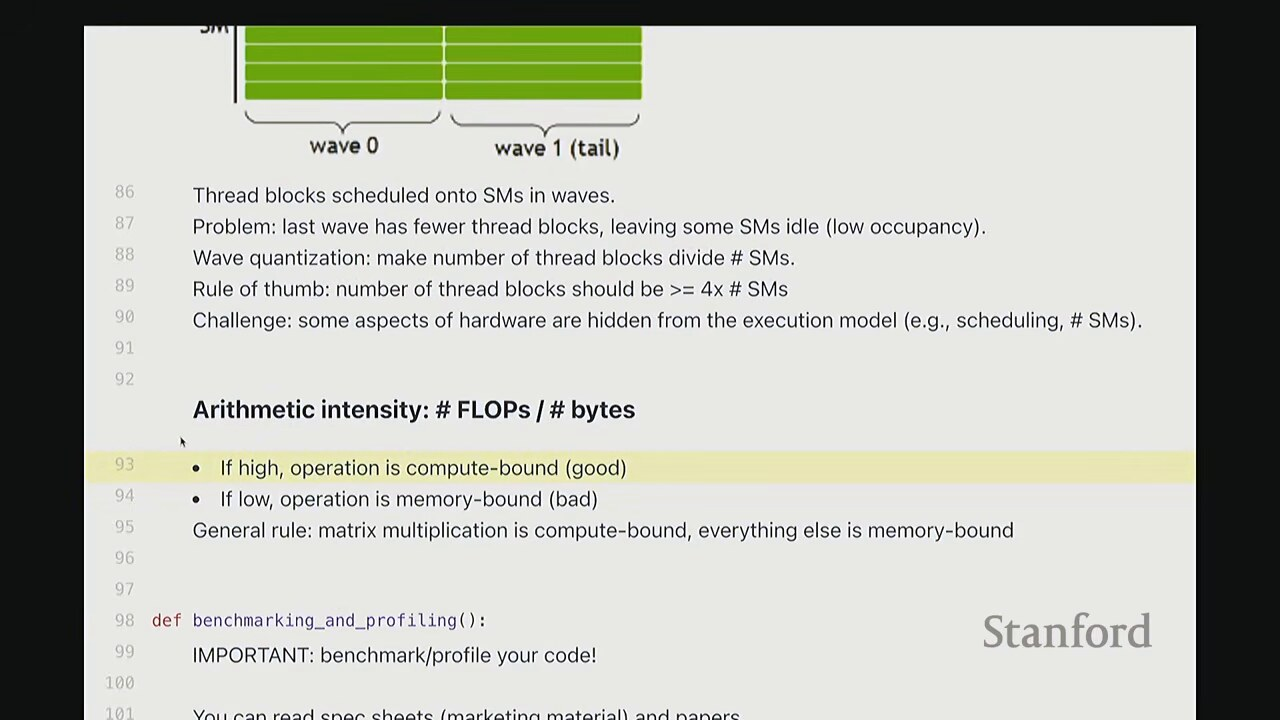
\includegraphics[width=\textwidth]{figures/fig_04_arithmetic_intensity.jpg}
\caption{算术强度与 roofline 模型：FLOPs/Byte 比率决定一个算子是 compute-bound 还是 memory-bound\protect\footnotemark}
\end{figure}
\footnotetext{视频画面时间区间：00:05:15--00:05:30。}

\textbf{算术强度（arithmetic intensity）}是本讲乃至整个 GPU 编程最重要的概念之一：我们希望 FLOPs 数相对于内存搬运字节数尽可能高。原因是上一讲展示过的 scaling 曲线——\emph{算力的增长速度远快于内存带宽的增长速度}，所以绝大多数运算最终都会变成\textbf{memory-bound}（被内存卡住），而不是 compute-bound。

\[
\text{arithmetic intensity} = \frac{\text{FLOPs}}{\text{Bytes transferred}}
\]

一个算子是否被内存卡住，由算术强度与机器的\textbf{平衡点（balance point）}比较决定：

\[
\text{balance point} = \frac{\text{peak FLOPs/s}}{\text{peak Bytes/s}}
\]

若算术强度 $<$ 平衡点，则 memory-bound；否则 compute-bound。

\begin{warningbox}{经验法则：矩阵乘是 compute-bound，其它几乎都是 memory-bound}
"如果做得巧妙，矩阵乘法是 compute-bound 的；其它所有东西基本都是 memory-bound 的。"——所以我们的任务就是想方设法减少 memory-bound 程度，或减轻其后果。这正是后面 kernel fusion、FlashAttention 等技巧的根本动机。
\end{warningbox}

\section{Benchmarking：如何正确测量时间}

\subsection{为什么不能凭直觉}

\begin{figure}[H]
\centering
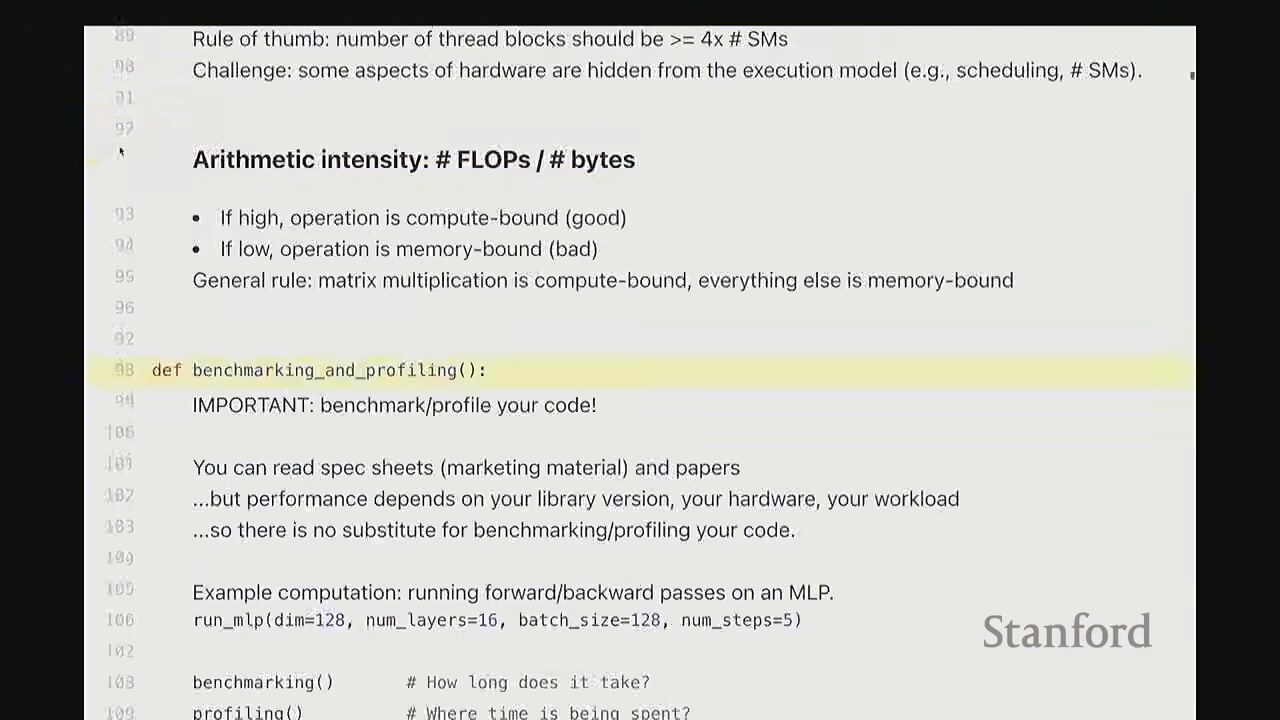
\includegraphics[width=\textwidth]{figures/fig_05_why_profile.jpg}
\caption{不要凭直觉猜瓶颈：理论能推到 roofline，但具体多快得靠 end-to-end benchmarking\protect\footnotemark}
\end{figure}
\footnotetext{视频画面时间区间：00:07:00--00:07:15。}

本讲的高层 take-home 只有一条：\textbf{想写高性能代码，就必须 benchmark 和 profile}。讲师见过太多学生（甚至工程师）"我觉得这里是瓶颈，于是花了三小时去优化它"，结果发现根本不是瓶颈——三小时纯属浪费。理论只能帮你推到 roofline 这种粗粒度结论；至于"你的矩阵乘到底多快"，它取决于库版本、硬件、各种 micro-architectural 细节，\emph{你最终只能靠 end-to-end benchmarking}。

\begin{practicebox}{本节的核心方法论}
先 benchmark（测量总耗时） $\rightarrow$ 再 profile（看时间花在哪） $\rightarrow$ 针对真正的瓶颈动手。顺序不能反。
\end{practicebox}

\subsection{示例：一个最小的 MLP}

\begin{figure}[H]
\centering
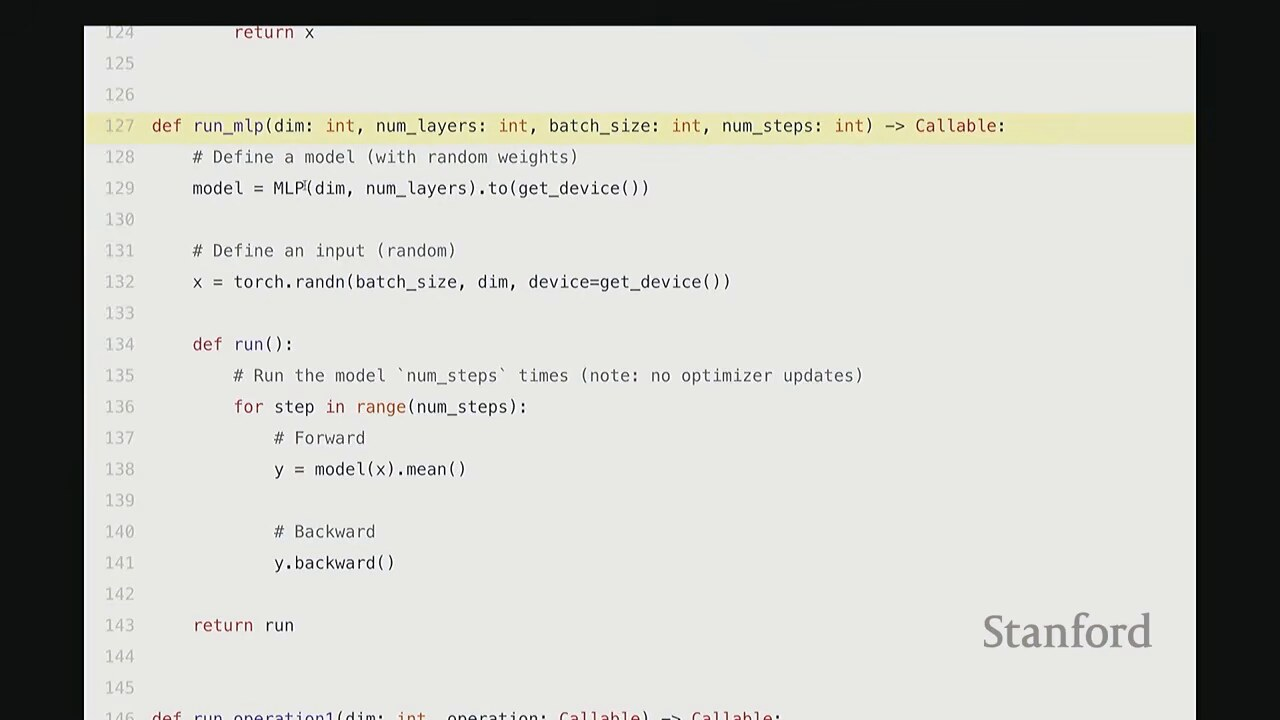
\includegraphics[width=\textwidth]{figures/fig_06_mlp_code.jpg}
\caption{示例 MLP：128 维、16 层，Linear 与 GELU 交替堆叠，前向 + 反向跑 5 步\protect\footnotemark}
\end{figure}
\footnotetext{视频画面时间区间：00:09:00--00:09:15。}

讲师用一个极简 MLP 作为运行示例：128 维、16 层、若干 batch size，跑 5 步前向+反向。结构就是 \texttt{Linear → GELU → Linear → GELU → \dots} 全部方阵。它简单到人人都能看懂，又复杂到足以暴露真实性能问题。

\subsection{benchmark() 包装函数}

\begin{figure}[H]
\centering
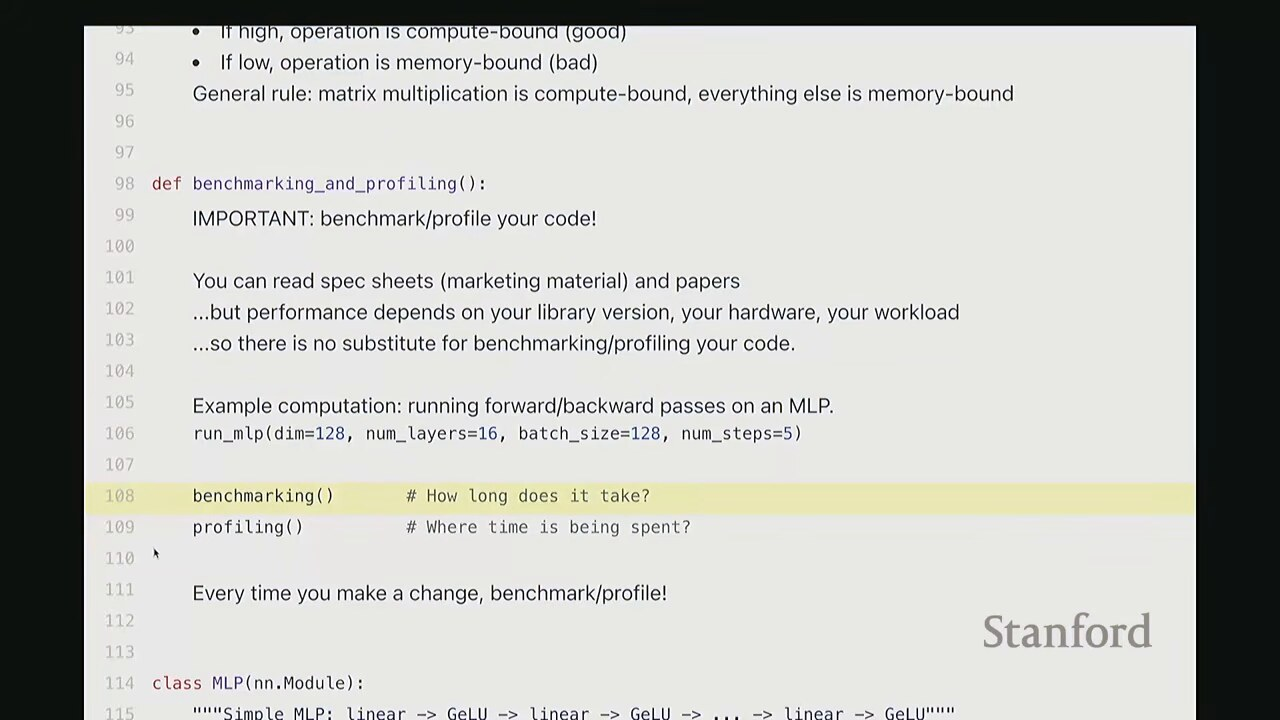
\includegraphics[width=\textwidth]{figures/fig_07_benchmark_fn.jpg}
\caption{\texttt{benchmark()} 函数：warm-up 迭代 + 多次 trials + 取均值返回毫秒数\protect\footnotemark}
\end{figure}
\footnotetext{视频画面时间区间：00:10:45--00:11:00。}

benchmarking 就是测一段操作的\textbf{wall-clock time}。讲师封装了一个 \texttt{benchmark(run, warmup, trials)} 函数，有两个看似啰嗦但绝对不能省的关键点。最终返回的是多次试验的均值：

\[
\bar{t} = \frac{1}{n}\sum_{k=1}^{n} t_k, \qquad t_k = \text{wall-clock of trial } k
\]

\begin{figure}[H]
\centering
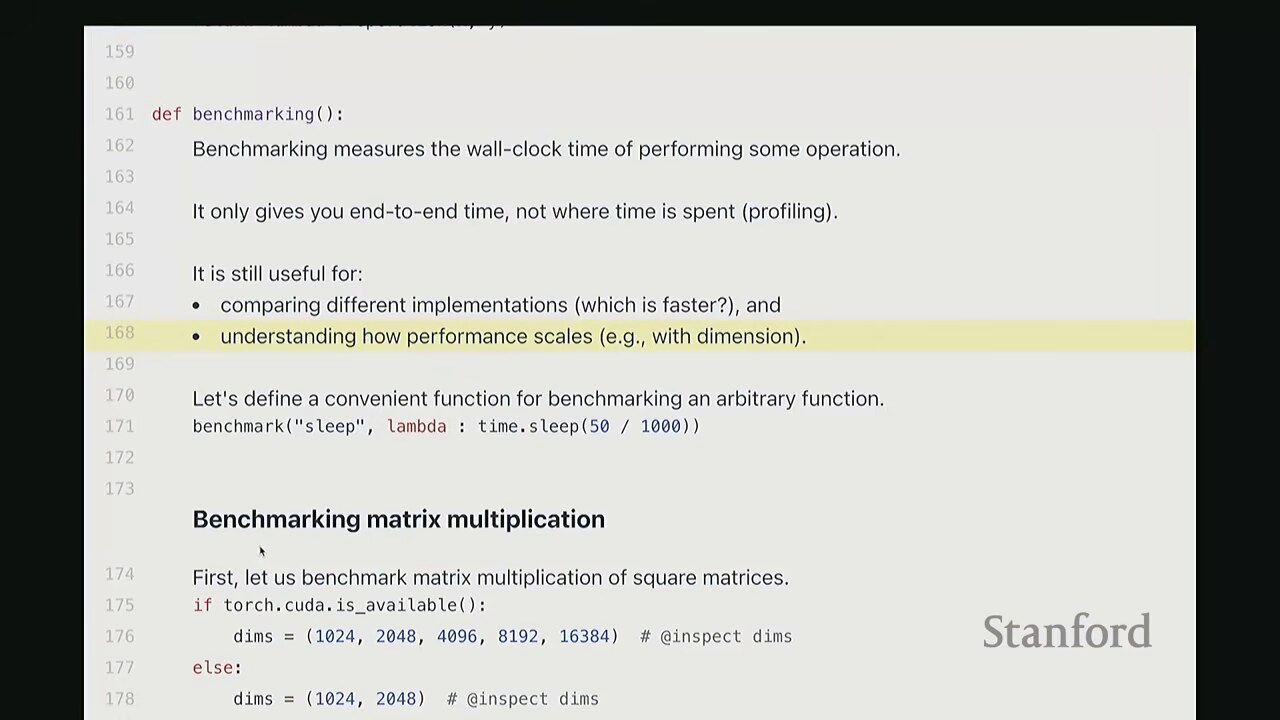
\includegraphics[width=\textwidth]{figures/fig_08_warmup_sync.jpg}
\caption{warm-up 与 \texttt{torch.cuda.synchronize()} 的必要性：CPU/GPU 是两个独立设备\protect\footnotemark}
\end{figure}
\footnotetext{视频画面时间区间：00:11:45--00:12:00。}

\begin{importantbox}{benchmark 的两个铁律}
\begin{enumerate}
    \item \textbf{Warm-up（预热）}：第一次执行 PyTorch 代码时，后台会做大量初始化——机器码编译、指令送进 GPU、各种 setup。你必须先跑几次 warm-up 迭代把这一切"消化掉"，再去测\emph{稳态}速度，否则你测到的其实是"启动开销"，而不是真实性能。
    \item \textbf{\texttt{torch.cuda.synchronize()}}：CPU 和 GPU 是两个\emph{独立}的计算单元。Python 代码在 CPU 上跑，它把 CUDA kernel "派发"给 GPU 后\textbf{不会等}，而是继续往下走。所以如果你直接在 \texttt{run()} 前后 \texttt{time.time()}，你测到的可能只是"CPU 把命令塞进队列"的时间，GPU 根本还没开始算！\texttt{synchronize()} 强制 CPU 等 GPU 把队列里所有 kernel 都跑完，二者状态对齐。
\end{enumerate}
\end{importantbox}

\begin{warningbox}{忘记 synchronize 的后果}
你会得到荒谬的数字——比如"我的巨型矩阵乘瞬间完成"。这绝对不是真的，只是 CPU 把 kernel 塞进队列后立刻返回了。\texttt{torch.cuda.Event} 或 \texttt{torch.cuda.synchronize()} 是修正这个问题的标准做法。
\end{warningbox}

最后多次重复取均值，因为单次测量会受 GPU 热节流（thermal throttling）等随机因素干扰。

\subsection{矩阵乘与 MLP 的 scaling}

\begin{figure}[H]
\centering
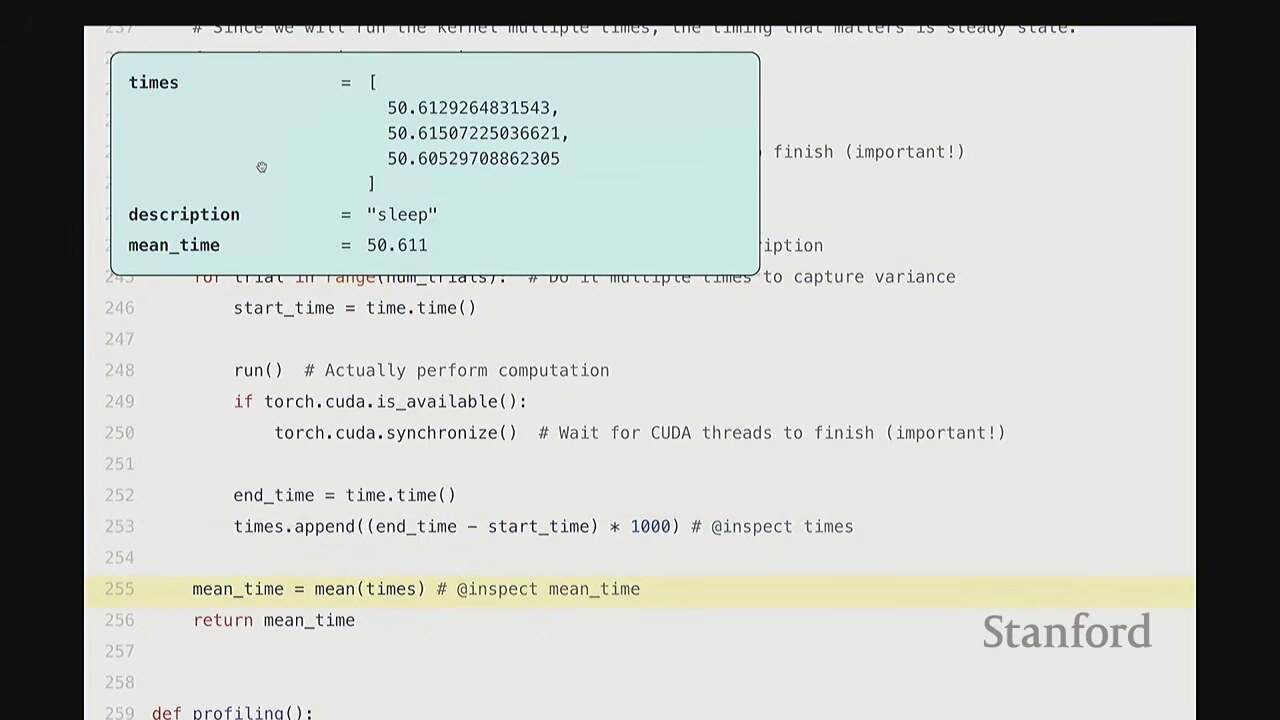
\includegraphics[width=\textwidth]{figures/fig_09_matmul_scaling.jpg}
\caption{矩阵乘规模 vs 运行时间：超线性 scaling；小矩阵因 kernel launch 常数开销几乎不变\protect\footnotemark}
\end{figure}
\footnotetext{视频画面时间区间：00:14:15--00:14:30。}

在课堂 H100 上跑矩阵乘，可见运行时间随矩阵规模\textbf{超线性}增长。但注意一个细节：在最小的尺寸（1024、2048）处，时间几乎不变——因为这里被\textbf{常数开销}（kernel launch、CPU→GPU 派发）主导，而不是计算本身。对 MLP 而言，无论增加 step 数还是层数，运行时间都呈\emph{线性} scaling（每步约 5 秒、每层约 5 秒），完全符合预期。

\section{Profiling：钻进函数内部}

\subsection{benchmark 太粗，profile 才能看到瓶颈}

\begin{figure}[H]
\centering
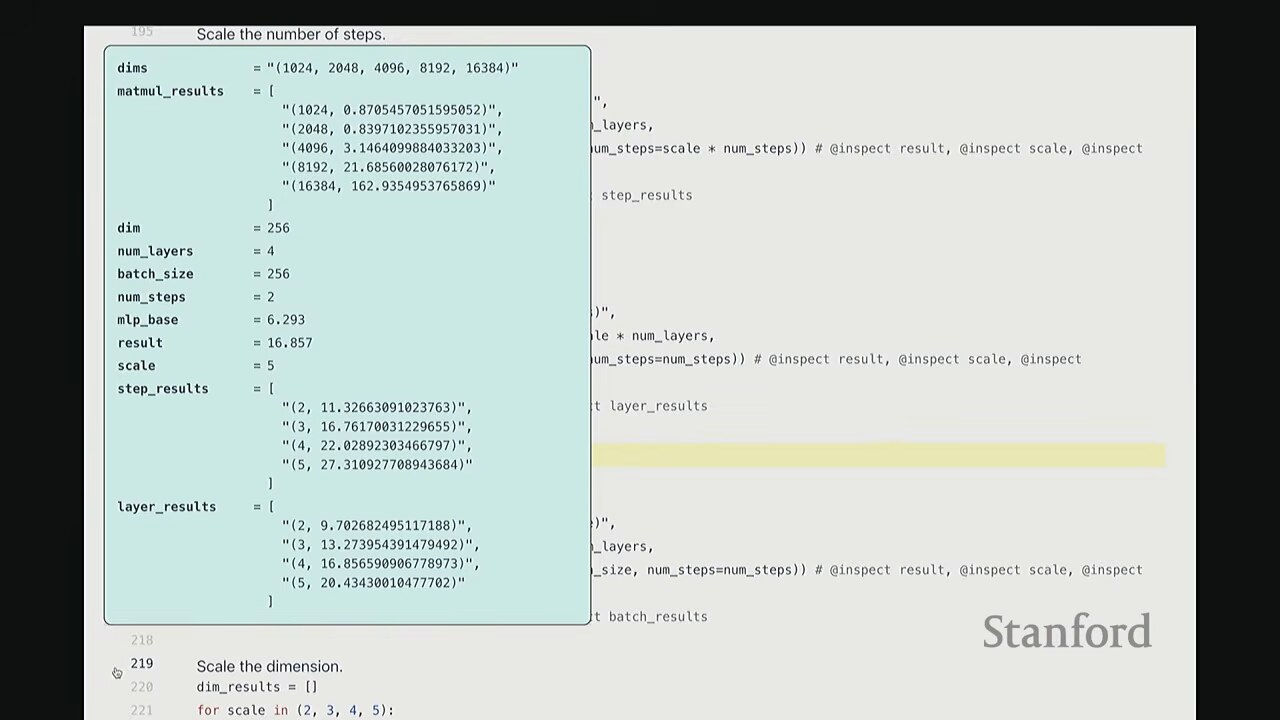
\includegraphics[width=\textwidth]{figures/fig_10_profiling_intro.jpg}
\caption{Profiling 比 benchmark 细粒度得多：能看穿 PyTorch 接口，直到底层 CUDA 调用\protect\footnotemark}
\end{figure}
\footnotetext{视频画面时间区间：00:18:15--00:18:30。}

benchmark 只告诉你"慢"，但不告诉你\emph{慢在哪}。而且你平时交互的只是 PyTorch Python 接口（比如 \texttt{a + b}），它底下还藏着一整个 CUDA 宇宙。\textbf{Profiling} 能让你一路看到最底层的调用，从而建立对"硬件到底在干什么"的直觉。

\begin{figure}[H]
\centering
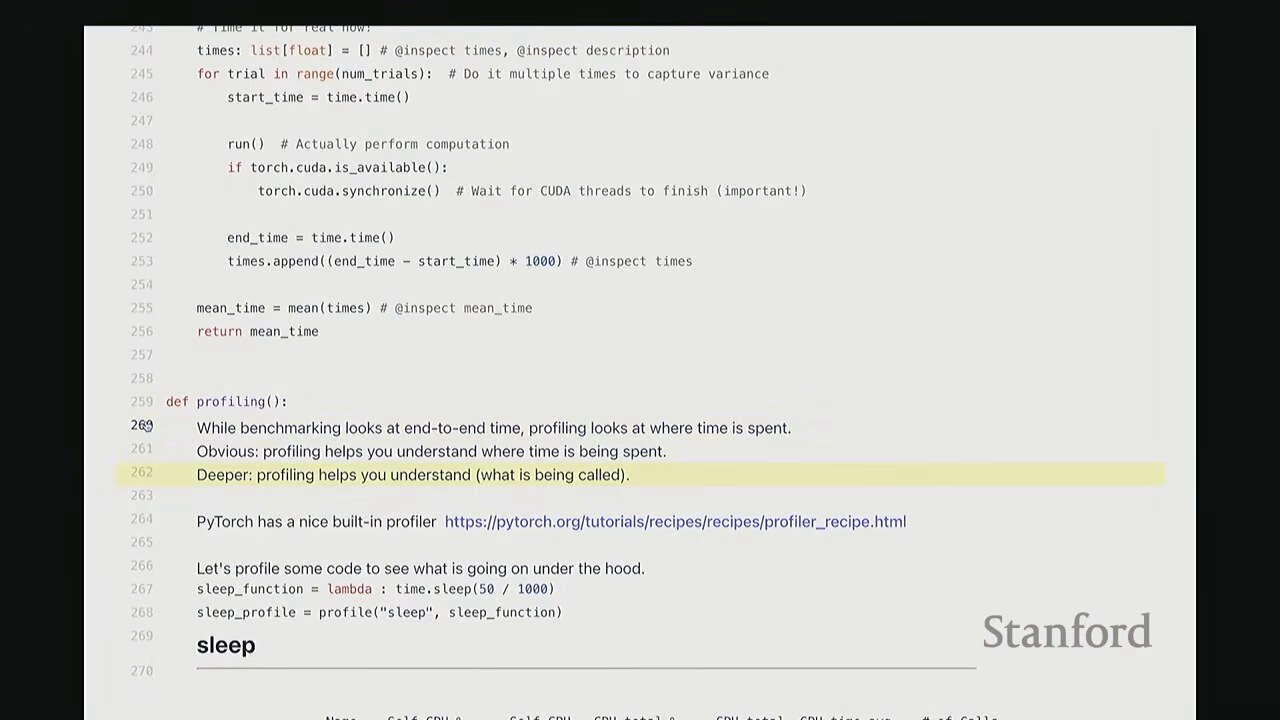
\includegraphics[width=\textwidth]{figures/fig_11_pytorch_profiler.jpg}
\caption{\texttt{torch.profiler}：内置 profiler，无需离开 Python/PyTorch 世界即可得到合理输出\protect\footnotemark}
\end{figure}
\footnotetext{视频画面时间区间：00:19:15--00:19:30。}

PyTorch 自带一个很好用的 \texttt{torch.profiler}，你不必离开 Python 世界就能拿到不错的输出。它同时追踪 CPU 和 GPU 时间，最终打印一张平均耗时表。

\subsection{从 add 到 mm：profile 一个简单算子}

\begin{figure}[H]
\centering
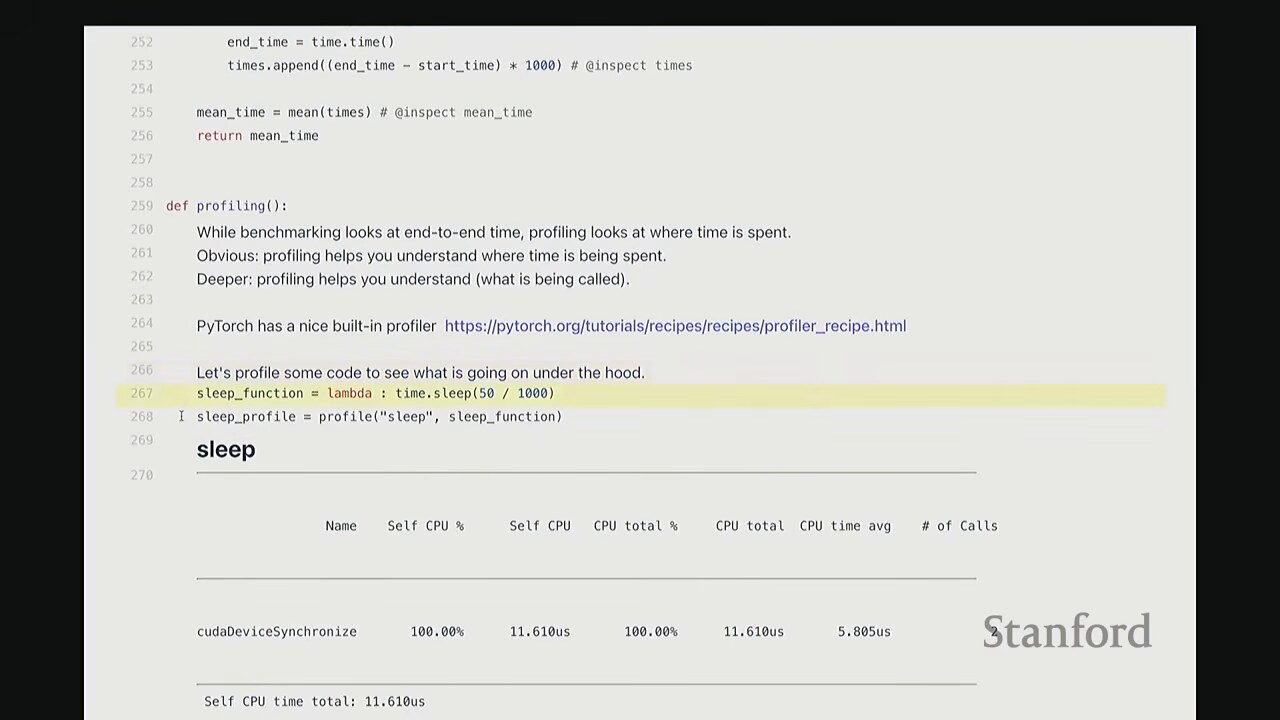
\includegraphics[width=\textwidth]{figures/fig_12_add_profile.jpg}
\caption{向量加法的 profile：\texttt{aten::add} → \texttt{vectorized\_elementwise\_kernel} → CUDA launch + synchronize\protect\footnotemark}
\end{figure}
\footnotetext{视频画面时间区间：00:21:00--00:21:15。}

profile \texttt{a + b}（2048 维矩阵相加），表面看只是 \texttt{a + b}，"冰山之下"却是一长串调用：先经过 \texttt{aten::add}（PyTorch 的 C++ 接口，简称 ATen），再 dispatch 到具体的 \texttt{vectorized\_elementwise\_kernel}（这才是真正做加法的 CUDA kernel），然后还有 \texttt{cuda\_launch\_kernel}（CPU 把命令发给 GPU 的开销）和 \texttt{cudaDeviceSynchronize}（等 GPU 完成）。最终 CPU 总耗时 1.4 毫秒，而 GPU 只花了 17 微秒——\textbf{GPU 极快，CPU 反而慢}，开销主要花在 C++ 接口层和"往 GPU 送命令"这件事上。

\begin{figure}[H]
\centering
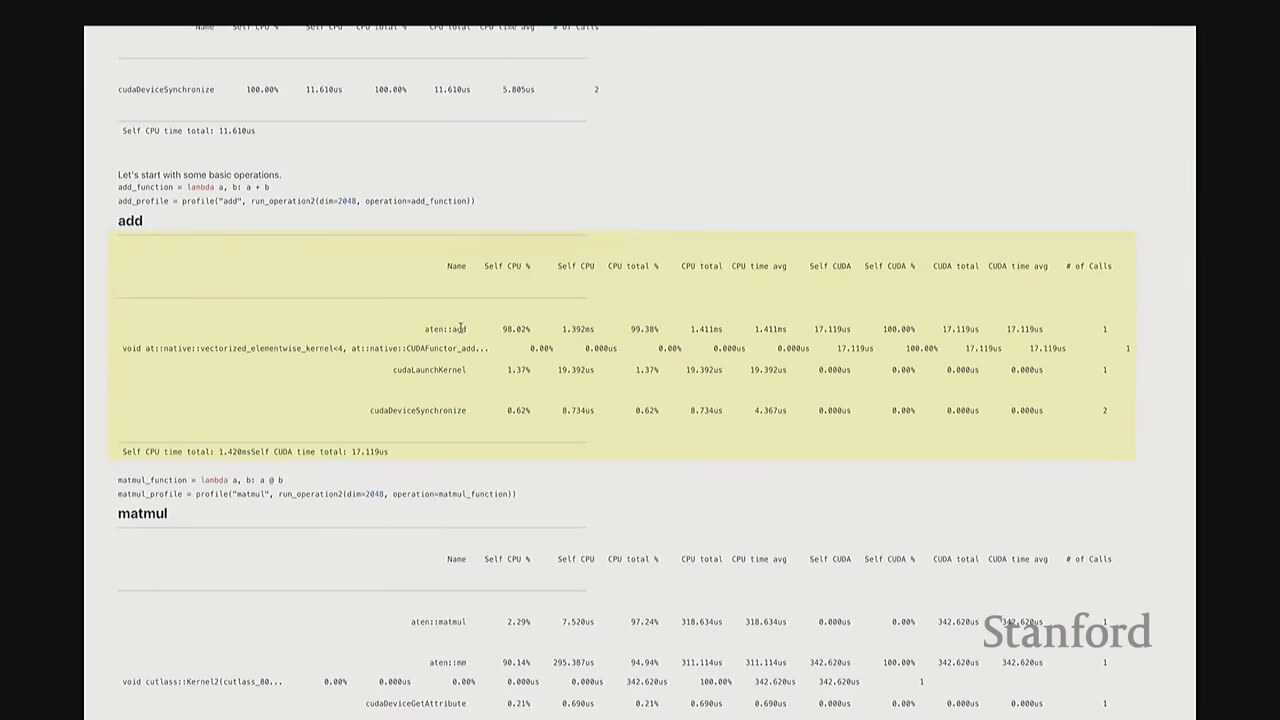
\includegraphics[width=\textwidth]{figures/fig_13_matmul_profile.jpg}
\caption{矩阵乘法的 profile：\texttt{aten::mm} → CUTLASS / XMMA GMM kernel，名字里含 tile size 与 block 数\protect\footnotemark}
\end{figure}
\footnotetext{视频画面时间区间：00:23:00--00:23:15。}

矩阵乘则更复杂：\texttt{aten::mm} 会 dispatch 到 NVIDIA 的高性能矩阵库 \textbf{CUTLASS}，kernel 名字里直接编码了 tile size、block 数等参数。注意\emph{不同尺寸的矩阵会 dispatch 到完全不同的 kernel}——128×128 的小矩阵直接走 \texttt{XMMA GMM}（不经 CUTLASS）。这正是 \texttt{torch.compile} 后来能"白捡 10\% 加速"的原因：它知道矩阵形状后，可以微基准测试并挑出当前硬件上最优的 matmul 子程序。

\begin{figure}[H]
\centering
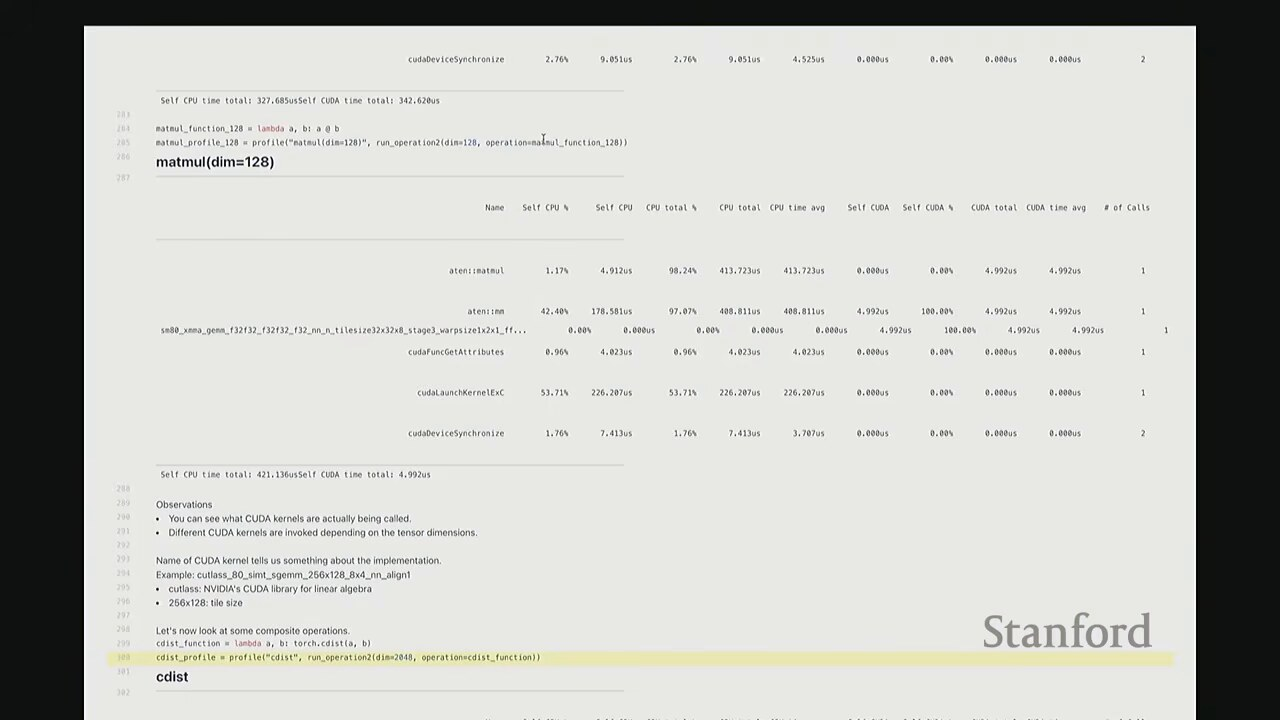
\includegraphics[width=\textwidth]{figures/fig_14_cdist_profile.jpg}
\caption{\texttt{torch.cdist} 的 profile：分解为 mm / pow / sum 等多个 CUDA kernel，按 GPU 时间占比排序\protect\footnotemark}
\end{figure}
\footnotetext{视频画面时间区间：00:27:00--00:27:15。}

\texttt{torch.cdist}（成对欧氏距离）是更复杂的算子：它被分解为 \texttt{aten::mm}、\texttt{aten::pow}、\texttt{aten::sum} 等多个底层调用，每个又对应一个 CUDA kernel。profile 表按 GPU 时间占比排序——比如 mm 占 78\%、拷贝/concat 占 6\%、pow 占 5\%、sum 占 3\%。这种"时间花在哪"的分解，正是优化决策的依据。

\subsection{GELU 与 softmax：已有融合 kernel}

\begin{figure}[H]
\centering
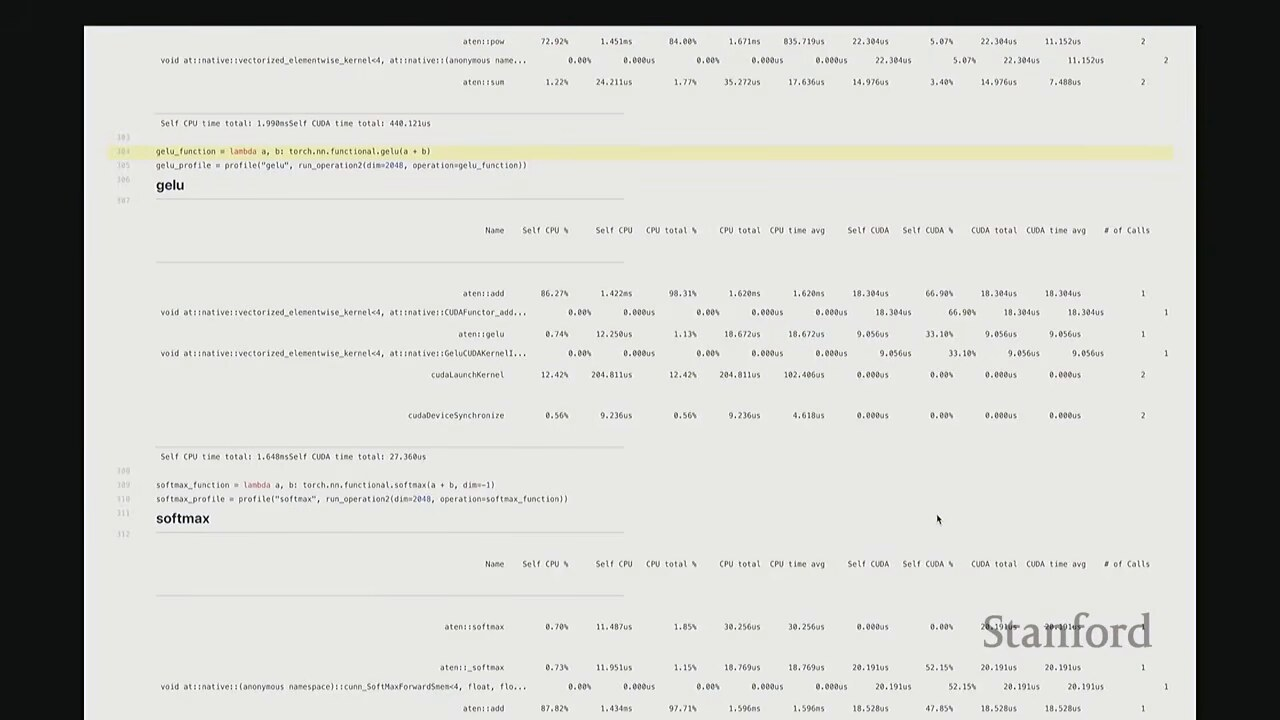
\includegraphics[width=\textwidth]{figures/fig_15_gelu_softmax_profile.jpg}
\caption{GELU / softmax 的 profile：这些核心原语已有\emph{融合好的单一 CUDA kernel}，不再 CPU/GPU 来回\protect\footnotemark}
\end{figure}
\footnotetext{视频画面时间区间：00:30:00--00:30:15。}

GELU 和 softmax 这类核心原语，PyTorch 内部已经写好了\textbf{融合算子}——一个 CUDA kernel 就把 tanh、exp、求和等全做完，不需要 CPU/GPU 之间来回。GELU 将作为本讲的"贯穿示例"。

\subsection{MLP 的 profile 与 Nsight Systems}

\begin{figure}[H]
\centering
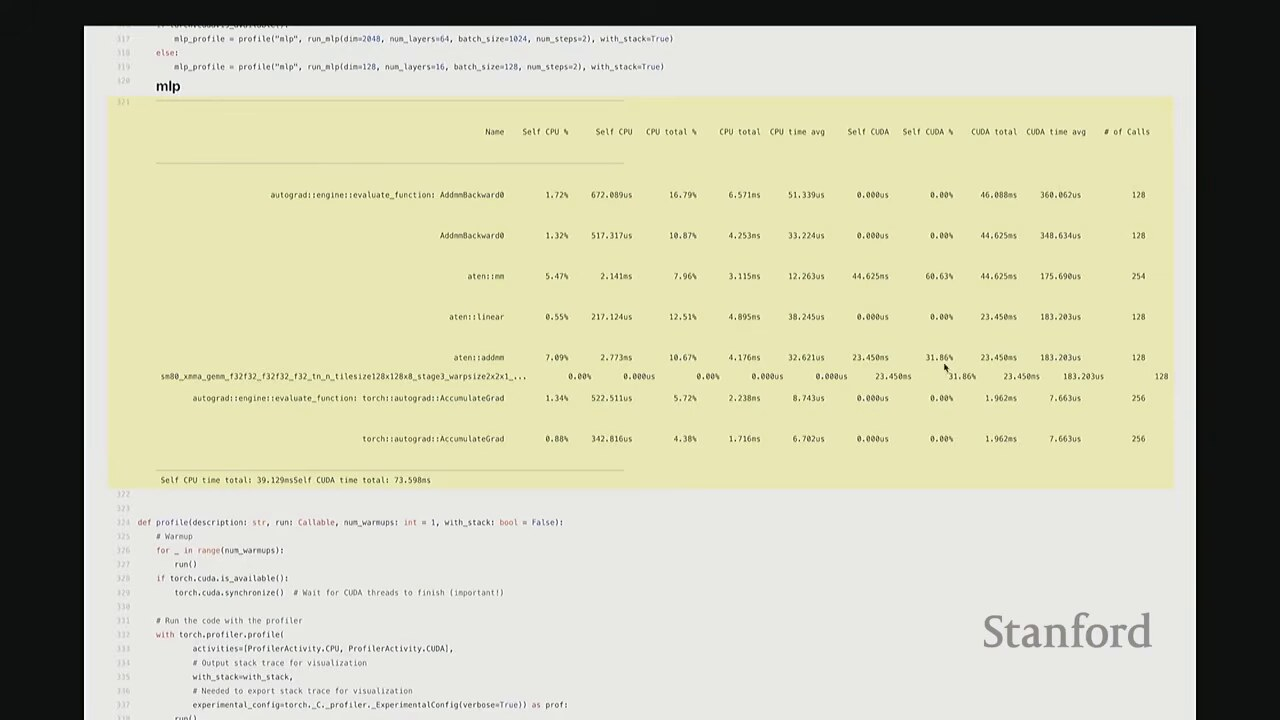
\includegraphics[width=\textwidth]{figures/fig_16_mlp_profile.jpg}
\caption{完整 MLP 的 \texttt{torch.profiler} 输出：可见 backward、mm、accumulate\_grad，但 31\% 时间去向成谜\protect\footnotemark}
\end{figure}
\footnotetext{视频画面时间区间：00:32:45--00:33:00。}

对完整 MLP 做 profile，能看到 backward、mm、accumulate\_grad 等操作，但有个尴尬：表里显示某项 \texttt{aten::mm} 占了 60\% 却\emph{没有对应的 kernel}！只显示前 10 行，对复杂模块这种视图力不从心。这时必须上"成年人用的 profiler"。

\begin{figure}[H]
\centering
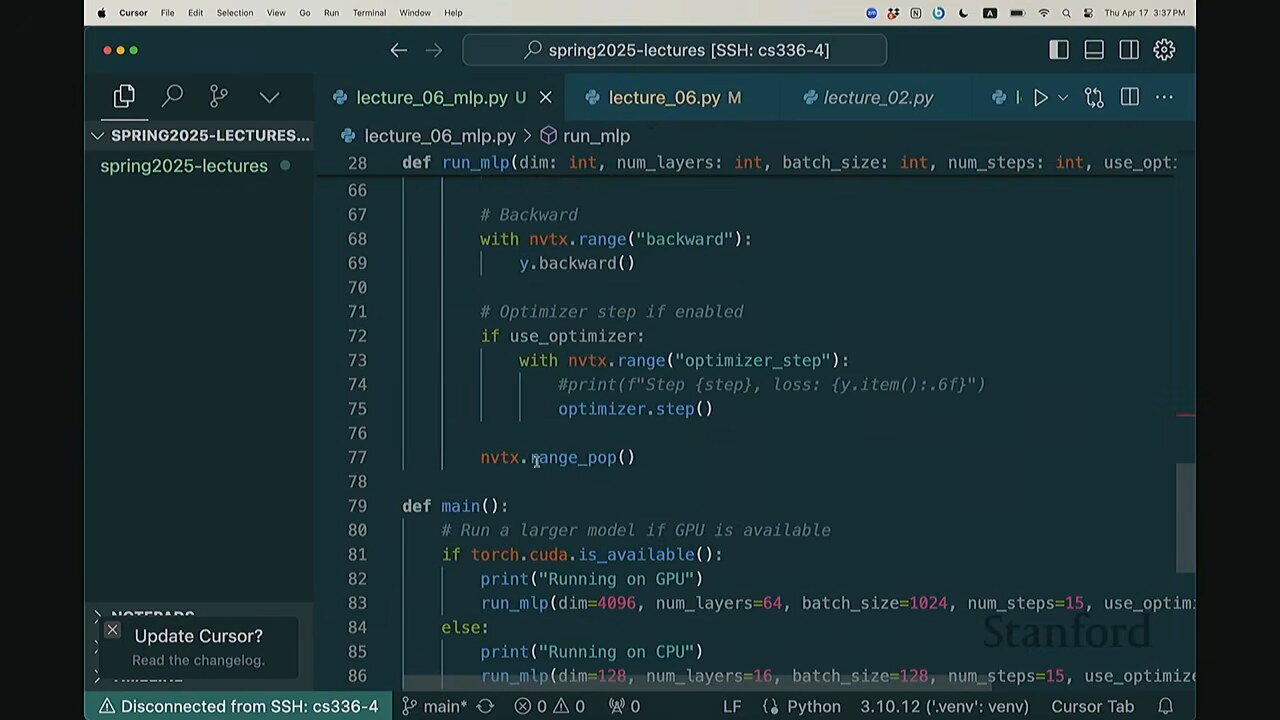
\includegraphics[width=\textwidth]{figures/fig_17_nsight_nvtx.jpg}
\caption{NVIDIA Nsight Systems：上半部分是 CUDA HW（GPU），下半部分是 threads（CPU），配 NVTX 标注\protect\footnotemark}
\end{figure}
\footnotetext{视频画面时间区间：00:34:45--00:35:00。}

\textbf{NVIDIA Nsight Systems（Nsight）}是查看 GPU 行为的工业级工具。它的视图分两半：上半是 \texttt{CUDA HW}（GPU 在干什么），下半是 \texttt{threads}（CPU 在干什么）。配合 \textbf{NVTX range 标注}（在 Python 代码里用 \texttt{nvtx.range\_push/pop} 把一段代码打上标签），profiler 就能在时间线上把"define model""step 0""step 1"等清晰地框出来。

\subsection{CPU 与 GPU 的异步执行}

\begin{figure}[H]
\centering
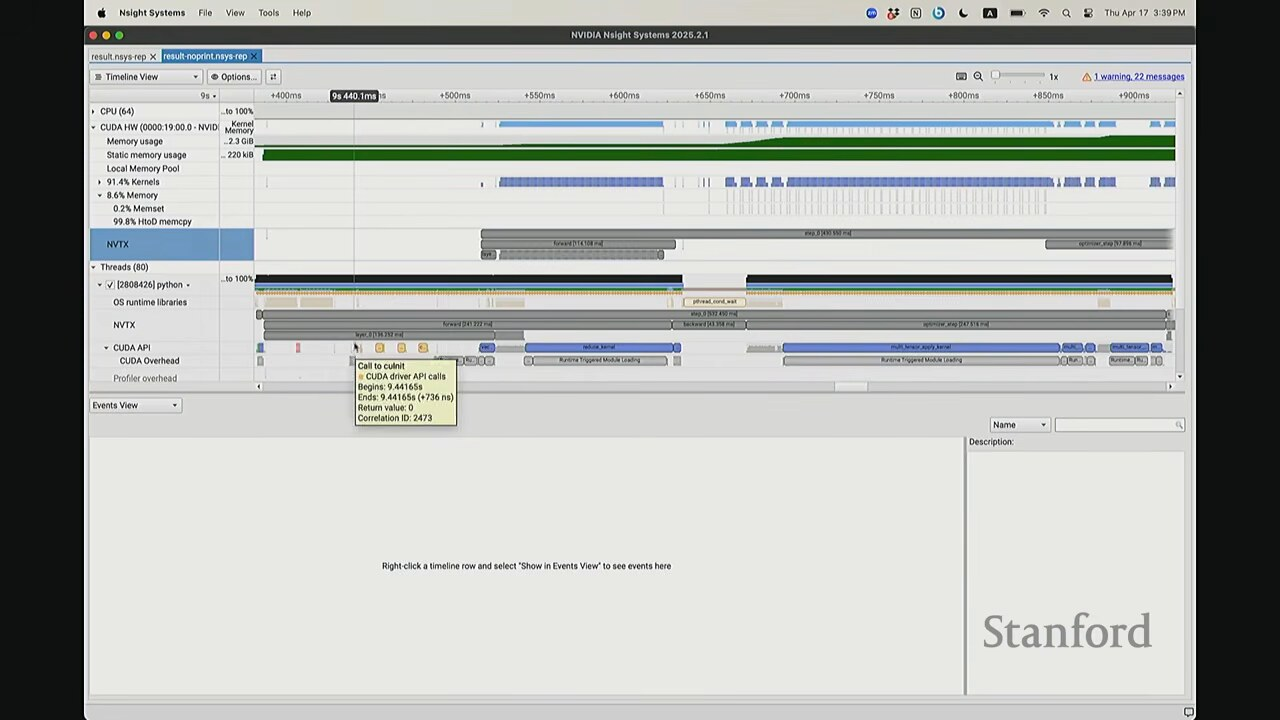
\includegraphics[width=\textwidth]{figures/fig_18_cpu_gpu_async.jpg}
\caption{CPU 跑得远比 GPU 快：CPU 在 layer 1 时，GPU 才刚到 layer 0；CPU 提前把 kernel 排进队列\protect\footnotemark}
\end{figure}
\footnotetext{视频画面时间区间：00:36:45--00:37:00。}

这是本讲最反直觉、也最重要的洞察之一。在 Nsight 时间线上可以看到：\textbf{CPU 跑得远比 GPU 快}。当 CPU 开始 layer 1 时，GPU 可能还在跑 layer 0；当 GPU 终于开始 layer 1 时，CPU 已经跑到 layer 9 了。CPU 的角色其实是\textbf{提前把 CUDA kernel 排进 GPU 的命令队列}："接下来跑这个、再跑这个、再跑这个……"直到队列深度（Q depth）填满才停下。

\begin{importantbox}{为什么 Python 这种"慢"语言也能榨干 GPU}
正是因为 CPU/GPU 解耦、CPU 可以远远跑在前面把命令排好队，所以\textbf{CPU 永远不是瓶颈}——这就是我们能用 Python 这种高层语言、却仍获得 GPU 满负荷利用的根本原因。Python 的慢，被异步流水线完全掩盖了。
\end{importantbox}

\subsection{一句 print 如何摧毁性能}

\begin{figure}[H]
\centering
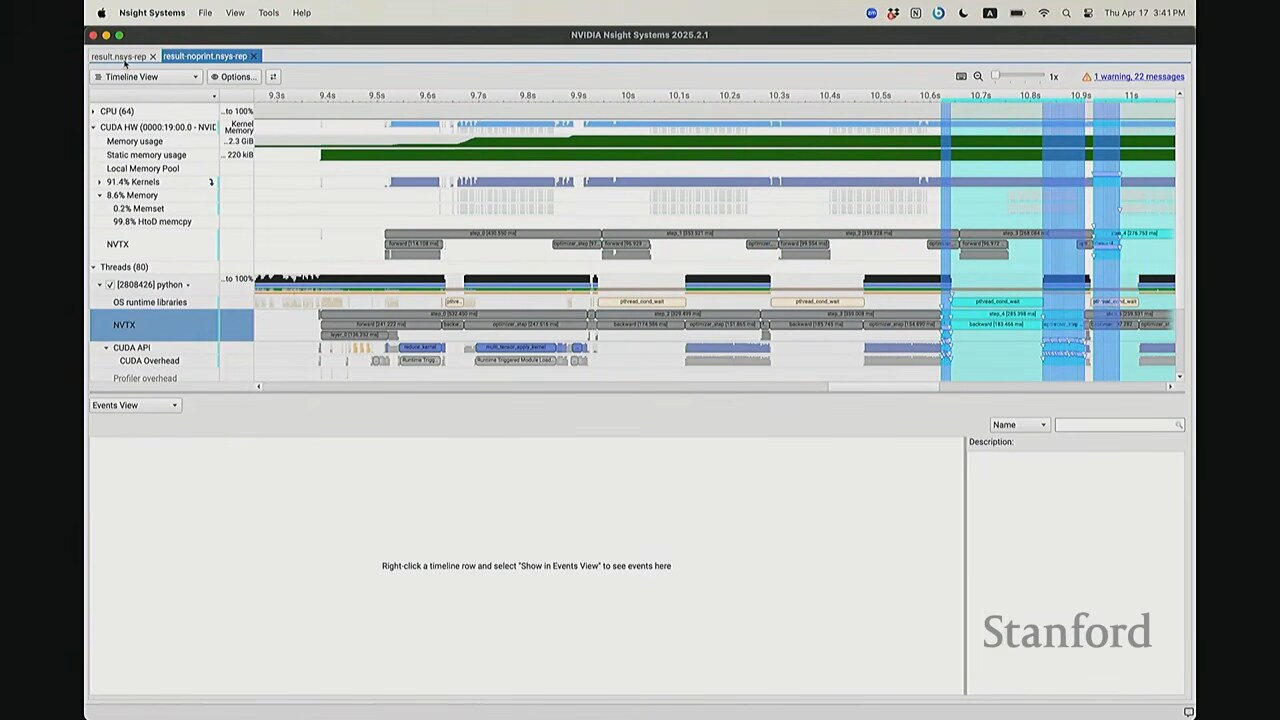
\includegraphics[width=\textwidth]{figures/fig_19_print_impact.jpg}
\caption{加一句 \texttt{print(loss)}：step 1 与 step 2 被迫对齐，CPU 必须等 GPU 算完 loss 才能打印\protect\footnotemark}
\end{figure}
\footnotetext{视频画面时间区间：00:38:45--00:39:00。}

一个看似无害的改动会带来巨大影响。假设你在训练循环里加了 \texttt{print(loss)}——"它只是个 print，能有多大影响？"但仔细想：要打印 loss，CPU 必须\emph{先拿到 loss 的值}，而 loss 还在 GPU 上没算完。于是 CPU 被迫 \texttt{cudaStreamSynchronize}，干等 GPU 把 backward 跑完。

\begin{figure}[H]
\centering
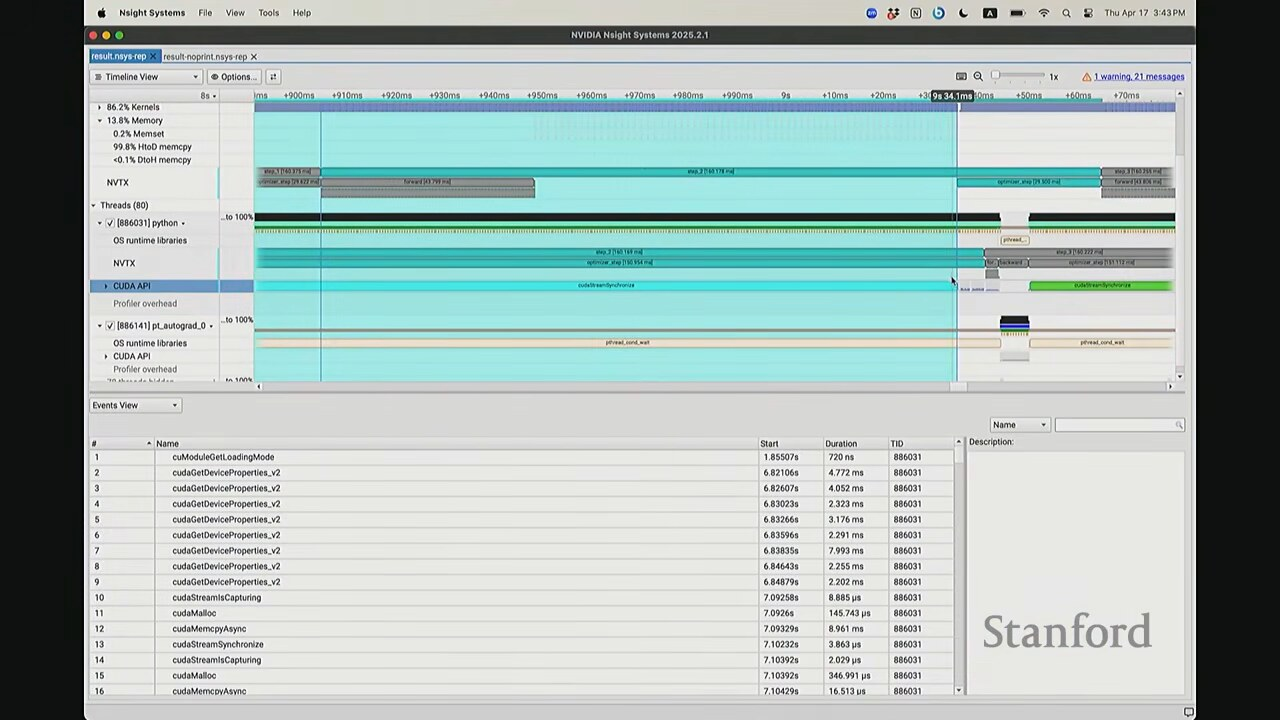
\includegraphics[width=\textwidth]{figures/fig_20_cuda_sync_wait.jpg}
\caption{\texttt{cudaStreamSynchronize}：CPU 空等 GPU 完成的"dummy 操作"，破坏异步流水线\protect\footnotemark}
\end{figure}
\footnotetext{视频画面时间区间：00:40:45--00:41:00。}

在 Nsight 上看得很清楚：加了 print 之后，step 1 和 step 2 几乎被\textbf{强制对齐}，CPU 没法再提前排队。虽然这里 GPU 利用率仍满（因为 backward 本身够重），但极端情况下（频繁打印、频繁同步），你会凭空制造一个 \textbf{CPU 瓶颈}——GPU 闲着等 CPU 派活。

\begin{warningbox}{性能反模式：训练循环里频繁 \texttt{.item()} / \texttt{print} / \texttt{.cpu()}}
任何把 GPU 张量"拉回 CPU"的操作都会触发 synchronize，破坏异步流水线。logging 要克制，最好攒一批再统一同步一次。
\end{warningbox}

\subsection{Nsight 的聚合视图与作业关联}

\begin{figure}[H]
\centering
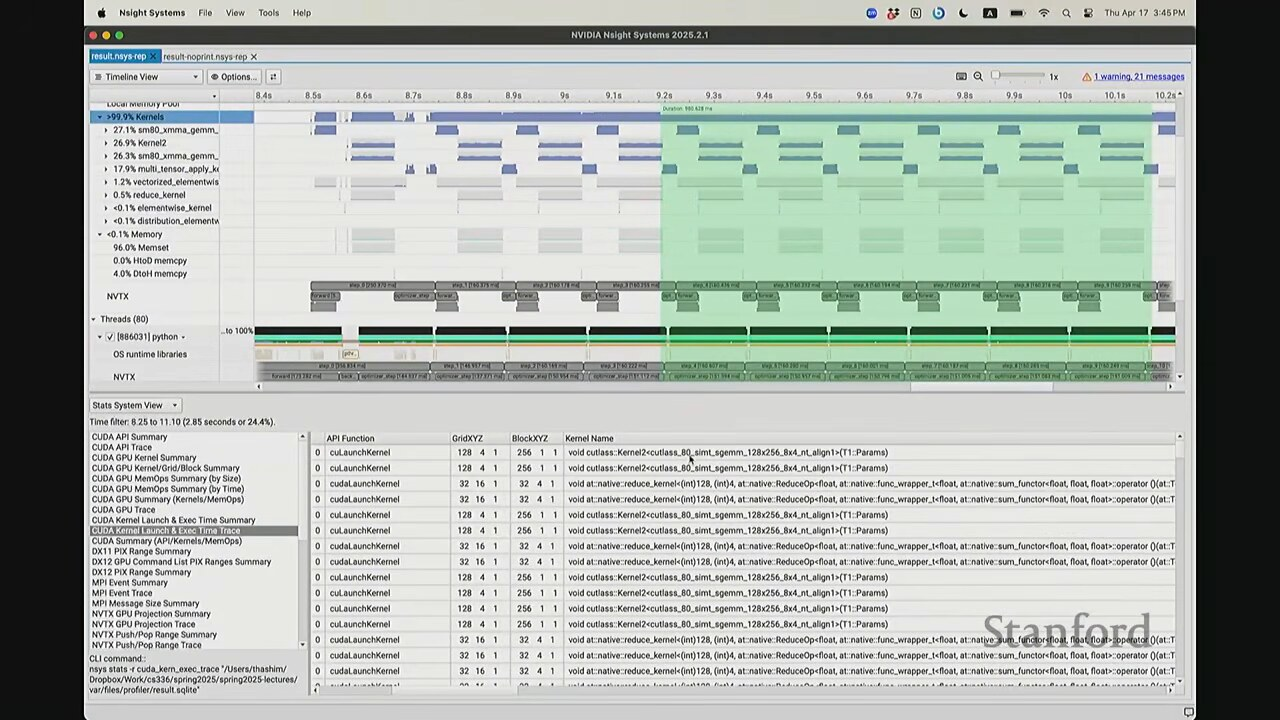
\includegraphics[width=\textwidth]{figures/fig_21_nsight_summary.jpg}
\caption{Nsight 的 kernel 执行摘要：按总时长排序，warm-up 排除前几步；可在 Assignment 2 里复用\protect\footnotemark}
\end{figure}
\footnotetext{视频画面时间区间：00:42:45--00:43:00。}

Nsight 还能聚合：框选一段 step（排除前几步 warm-up），看"CUDA kernel execution summary"按总时长排序，从而一眼定位最耗时的 kernel。Assignment 2 会让你亲手玩这个工具，建立对硬件行为的直觉。

\section{Kernel Fusion：为什么要自己写 kernel}

\subsection{工厂与仓库的比喻}

还记得之前讲过的 \textbf{kernel fusion（算子融合）}那张图吗？把它想象成工厂和仓库：每做一次运算，就要把数据从仓库（global memory）搬到工厂（SM），算完再搬回去。如果天真地连续做一串小运算，你就要为"来回搬运"付很多次代价。\textbf{正确的做法是把所有运算塞进一个工厂里一次性做完}，只搬一次。

\begin{knowledgebox}{Kernel fusion 的本质}
把多个小 kernel 融合成一个大 kernel，让中间结果留在寄存器/shared memory 里，避免反复读写 global memory。这直接提升 arithmetic intensity，把 memory-bound 的串算子变成接近 compute-bound 的单算子。
\end{knowledgebox}

\subsection{GELU：贯穿全讲的示例}

GELU（Gaussian Error Linear Unit，高斯误差线性单元）是本讲的贯穿示例。它的近似形式（也是 PyTorch 默认 \texttt{tanh} 近似）为：

\[
\mathrm{GELU}(x) \approx 0.5\,x\!\left(1 + \tanh\!\left[\sqrt{\tfrac{2}{\pi}}\,\left(x + 0.044715\,x^3\right)\right]\right)
\]

\begin{figure}[H]
\centering
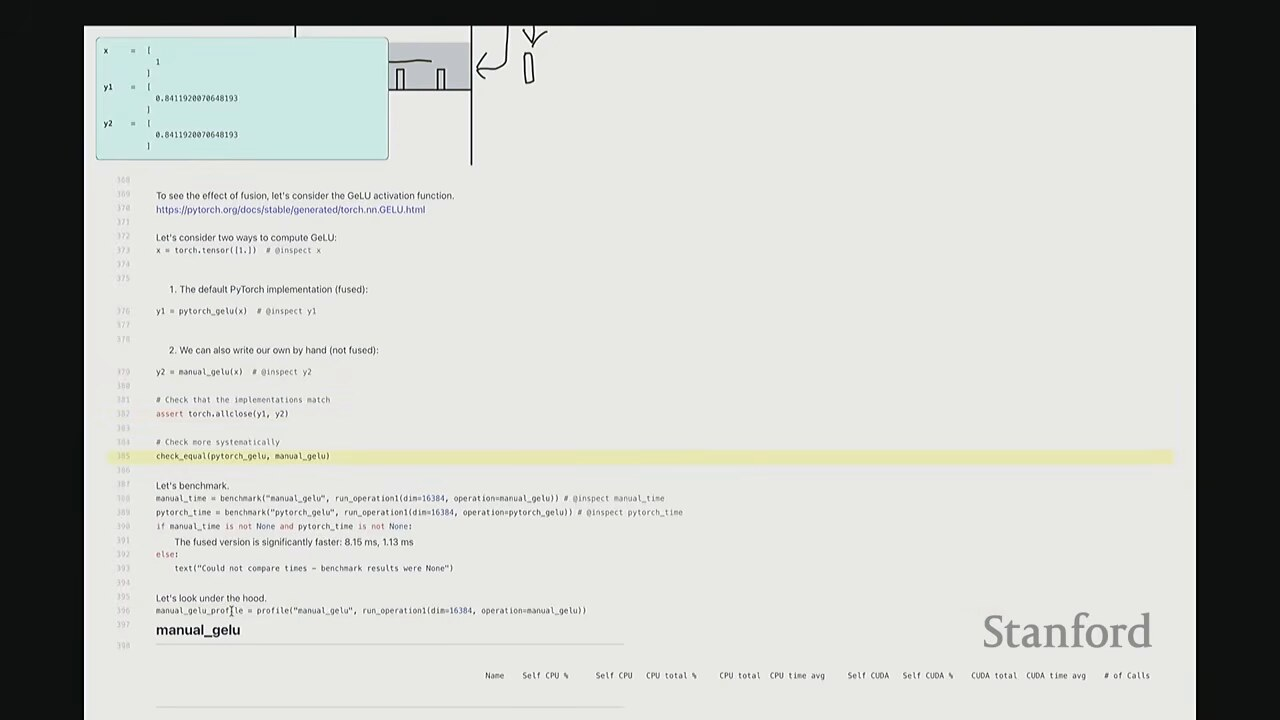
\includegraphics[width=\textwidth]{figures/fig_22_gelu_benchmark.jpg}
\caption{GELU 基准：naive 手写版 8.15 ms vs PyTorch 融合版 1.13 ms（约 8 倍差距）\protect\footnotemark}
\end{figure}
\footnotetext{视频画面时间区间：00:45:45--00:46:00。}

讲师先写了两种实现：PyTorch 官方的 \texttt{F.gelu(approximate='tanh')}，以及"naive 手写"——直接照公式 \texttt{0.5 * x * (1 + tanh(...))} 在 PyTorch 里展开。两者数值完全一致，但 benchmark 差距惊人：\textbf{手写版 8.1 毫秒，PyTorch 版 1.1 毫秒，差了 8 倍}。

为什么手写这么慢？因为展开后有 tanh、$x^3$、乘常数、加法、乘 0.5、乘 $x$ 等一连串运算，每个都触发一个独立的 CUDA kernel，数据在 global memory 和 SM 之间来回搬运。而 PyTorch 内部是一个\textbf{融合好的单 kernel}。我们的目标就是：从 8.1 毫秒逼近 1.1 毫秒。

\begin{importantbox}{本节的目标函数}
\[
\text{8.1 ms (naive)} \;\xrightarrow{\text{写 kernel}}\; \text{接近 1.1 ms (PyTorch 融合版)}
\]
接下来用三种方式（CUDA / Triton / torch.compile）逐一尝试。
\end{importantbox}

\section{手写 CUDA Kernel}

\subsection{CUDA 是 C++ API}

\begin{figure}[H]
\centering
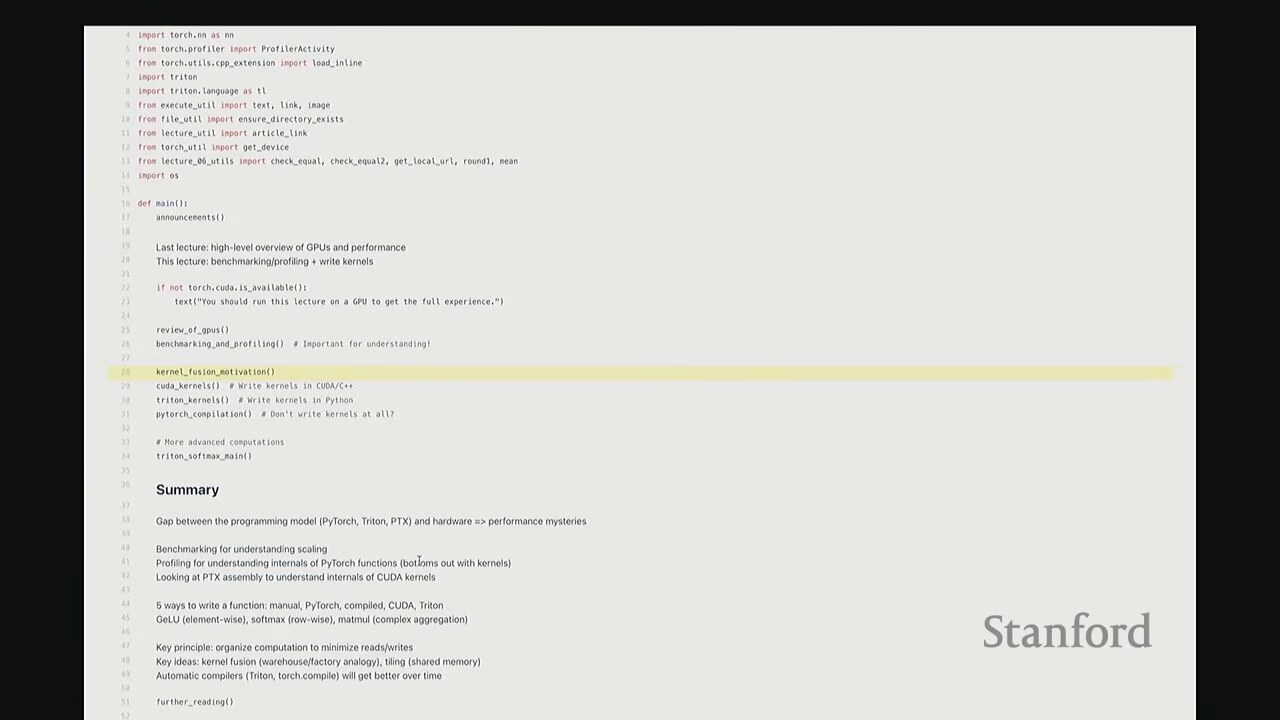
\includegraphics[width=\textwidth]{figures/fig_23_cuda_kernel_intro.jpg}
\caption{CUDA = 编程 GPU 的 C++ API；grid（block 集合）/ block（线程集合）/ thread 三级层次\protect\footnotemark}
\end{figure}
\footnotetext{视频画面时间区间：00:48:45--00:49:00。}

\textbf{CUDA 本质上是与 GPU 交互的 C++ API}。编程模型就是我们回顾过的层次结构：\textbf{grid}（一组 thread block 的集合）$\to$ \textbf{block}（一组线程，落在单个 SM）$\to$ \textbf{thread}（真正执行计算）。每个 kernel 函数会拿到三个坐标：\texttt{blockIdx}（我在哪个 block）、\texttt{blockDim}（block 有多大）、\texttt{threadIdx}（我在 block 内的偏移），由此算出自己负责的全局坐标 $i$，再决定要算什么。

\begin{practicebox}{调试 CUDA 的第一条命令}
启动前设环境变量 \texttt{CUDA\_LAUNCH\_BLOCKING=1}，让 kernel 同步执行、把错误信息及时返回 CPU。不这么干，你在 CUDA 里几乎没法调试——错误会异步冒出来，堆栈完全对不上。
\end{practicebox}

\subsection{GELU 的 CUDA 实现}

\begin{figure}[H]
\centering
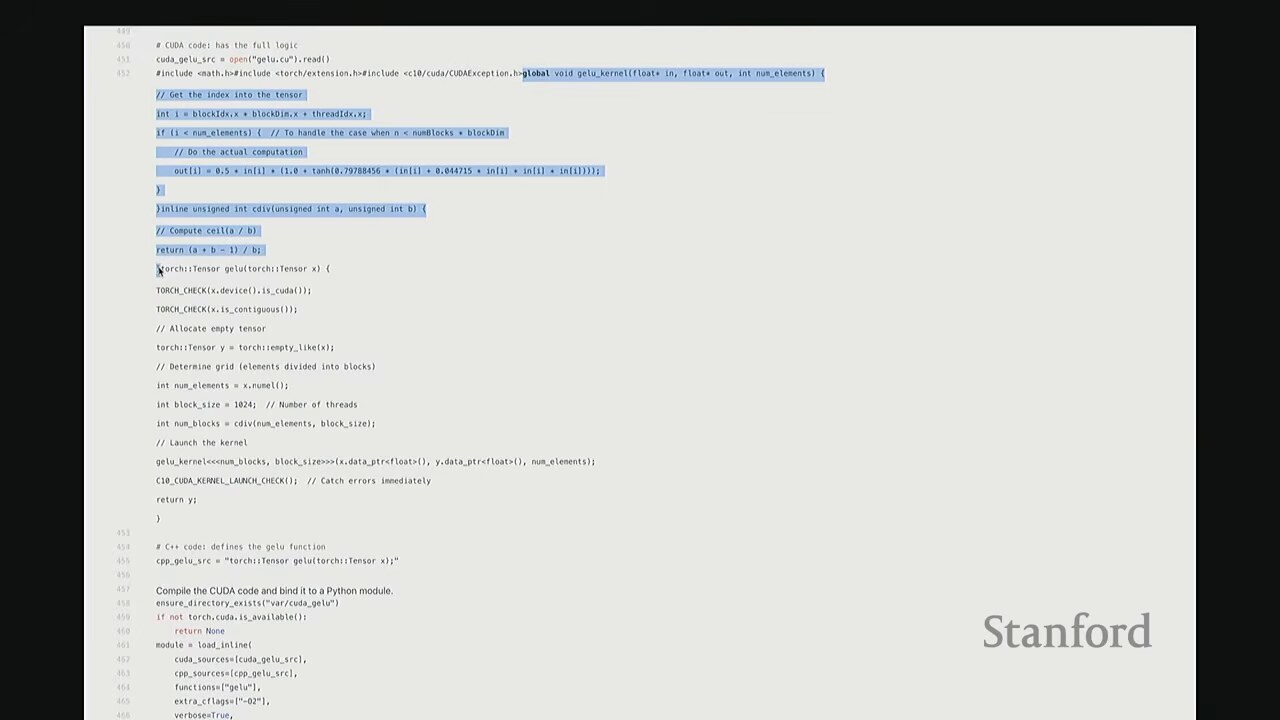
\includegraphics[width=\textwidth]{figures/fig_24_cuda_gelu_code.jpg}
\caption{CUDA GELU 完整代码：\texttt{\_\_global\_\_} kernel + CPU 侧 wrapper（contiguous 检查、\texttt{empty\_like}、\texttt{<<<>>>} 启动）\protect\footnotemark}
\end{figure}
\footnotetext{视频画面时间区间：00:51:45--00:52:00。}

代码分两部分。CPU 侧的 \textbf{wrapper（包装函数）}做编排：先 \texttt{assert x.is\_cuda}（确保数据在 GPU 上），再 \texttt{assert x.is\_contiguous()}（确保内存连续——因为我们要做指针算术，假设 $x$ 躺在一整块连续内存里）。然后用 \texttt{torch.empty\_like} 分配输出 $y$（注意不是 \texttt{zeros}，省一次清零，反正马上要写进去）。接着算 grid：\texttt{num\_elements}、\texttt{block\_size}、向上取整的 \texttt{num\_blocks}（保证最后一个不满的块也被覆盖），最后用 \texttt{gelu\_kernel<<<num\_blocks, block\_size>>>(x\_ptr, y\_ptr, n)} 启动。

\begin{figure}[H]
\centering
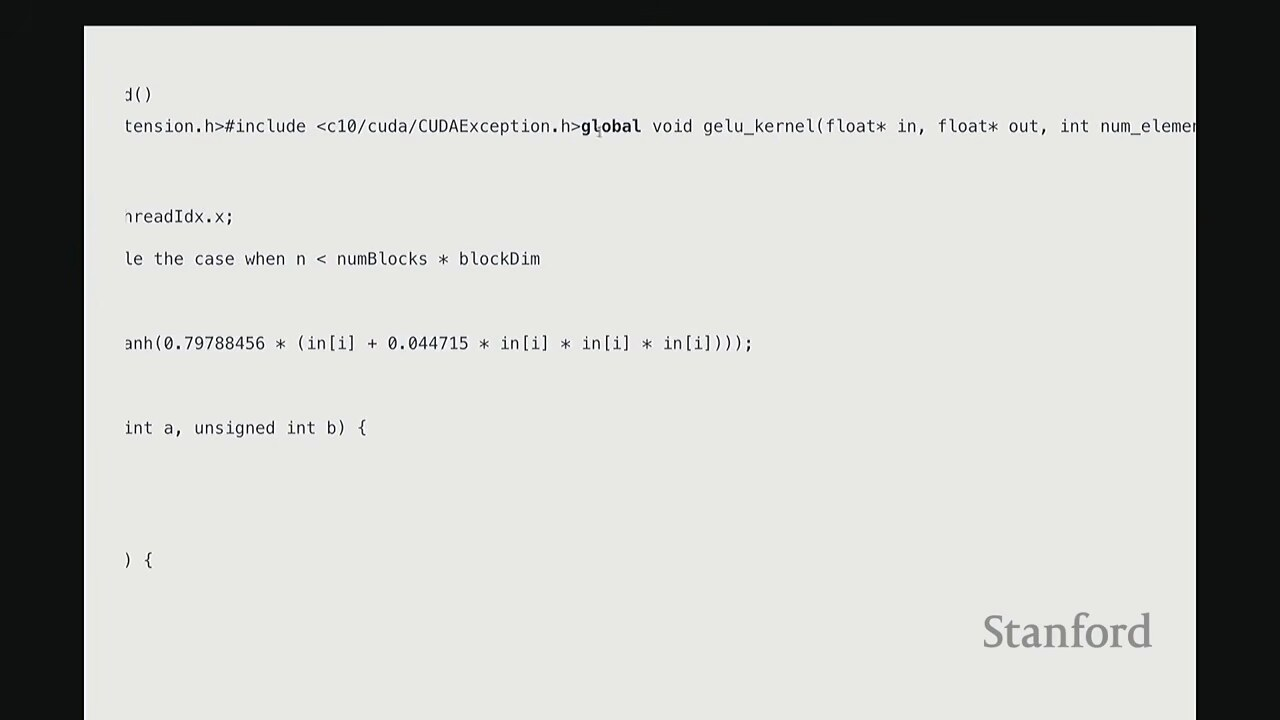
\includegraphics[width=\textwidth]{figures/fig_25_gelu_kernel_detail.jpg}
\caption{\texttt{\_\_global\_\_ void gelu\_kernel}：\texttt{blockIdx.x * blockDim.x + threadIdx.x} 算全局坐标、边界检查、套 tanh 公式\protect\footnotemark}
\end{figure}
\footnotetext{视频画面时间区间：00:55:00--00:55:15。}

GPU 侧的 \textbf{kernel 本体}用 \texttt{\_\_global\_\_} 关键字标记（标识"这是 CUDA kernel 函数"）。每个线程先算自己的全局下标：

\[
i = \text{blockIdx.x} \times \text{blockDim.x} + \text{threadIdx.x}
\]

\begin{itemize}
    \item \texttt{blockIdx.x}：我在第几个 block（乘以 block 大小得到本 block 的起点）。
    \item \texttt{threadIdx.x}：我在 block 内的偏移。
\end{itemize}

然后是\textbf{边界检查} \texttt{if (i < n)}——CUDA 没有内置越界保护，最后那个不满的 block 里有些线程会算到数组外，必须让它们什么都不做。最后套 GELU 公式 \texttt{out[i] = gelu(in[i])}，结束。整个 kernel 通过指针直接读写，无需关心拷贝细节。

\subsection{CUDA GELU 的性能}

\begin{figure}[H]
\centering
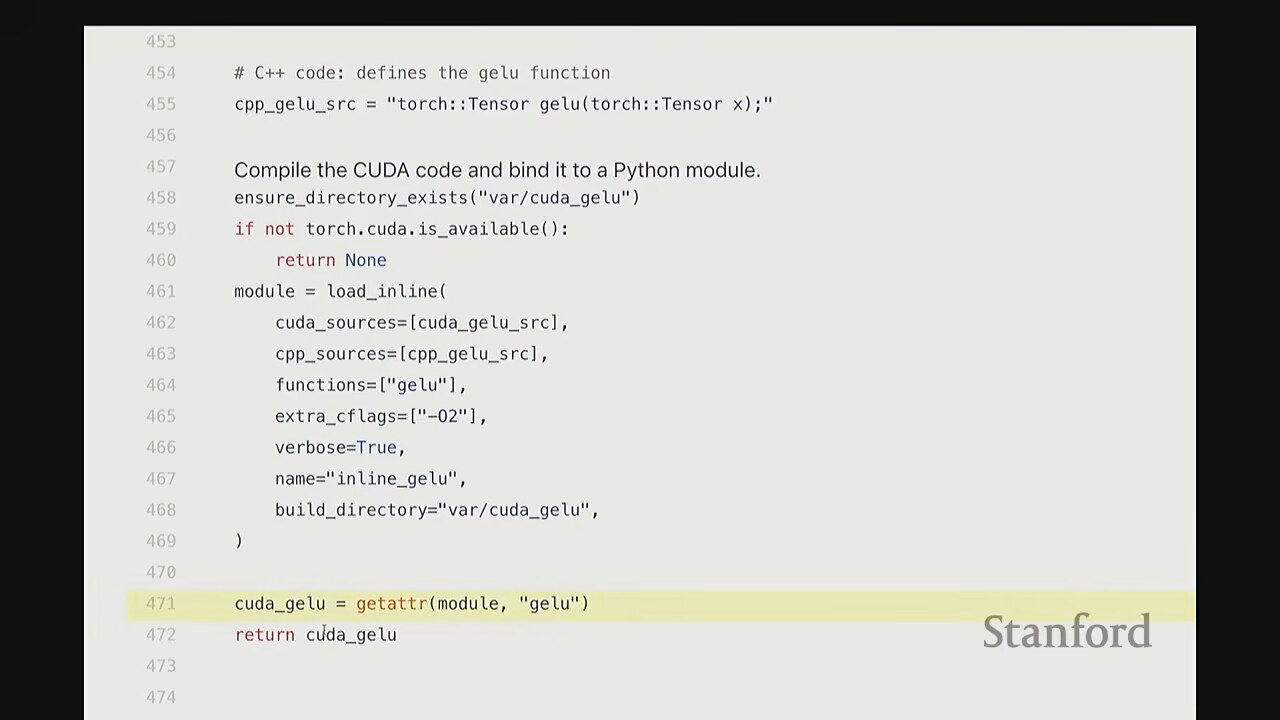
\includegraphics[width=\textwidth]{figures/fig_26_cuda_benchmark.jpg}
\caption{CUDA GELU 基准：1.84 ms（从 8.1 ms 降到接近 PyTorch 的 1.1 ms），单 kernel 占满 GPU 时间\protect\footnotemark}
\end{figure}
\footnotetext{视频画面时间区间：00:57:45--00:58:00。}

benchmark 结果：PyTorch 1.1 ms、naive 手写 8.1 ms、\textbf{我们的 CUDA 1.84 ms}——没追平 PyTorch，但已经从 8 ms 降到 1.8 ms，非常接近了，而且 C++ 代码并不难写。profile 也证实：现在只有一个 \texttt{gelu\_kernel} 占满 100\% GPU 时间，加上 \texttt{empty} / \texttt{empty\_strided} / \texttt{cuda\_launch\_kernel} / \texttt{cudaDeviceSynchronize} 等辅助调用。\textbf{kernel fusion 的问题已经被解决了}——所有算子融成了一个。

\begin{knowledgebox}{什么好写，什么不好写}
这种 element-wise 操作（每个元素独立计算）在 CUDA 里极其好写——你有新的激活函数，随手就能写一个。但更复杂的、需要\emph{读多个值做 reduction} 的操作（比如 FlashAttention）会麻烦得多，不过 Assignment 2 里你会亲手做。
\end{knowledgebox}

\section{Triton：Pythonic 的 GPU 编程}

\subsection{Triton 是什么}

\begin{figure}[H]
\centering
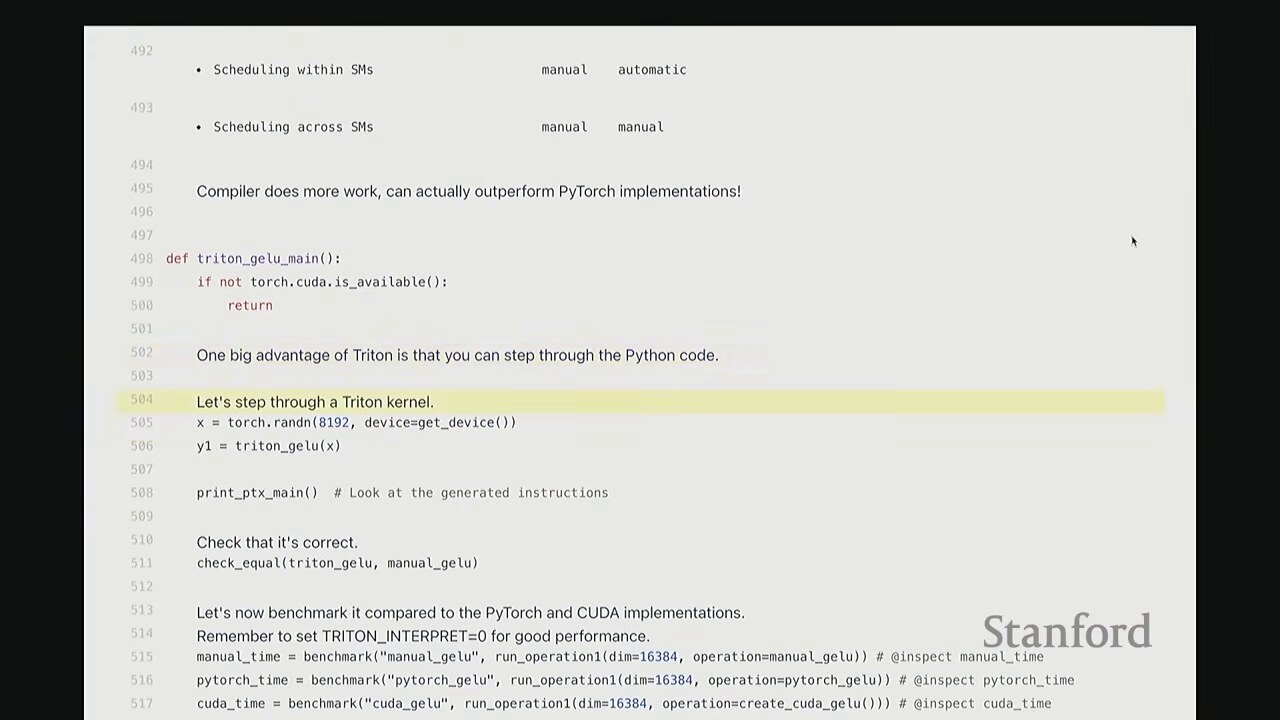
\includegraphics[width=\textwidth]{figures/fig_27_triton_intro.jpg}
\caption{Triton：OpenAI 2021 推出的 DSL，block 级编程，自动管理 coalescing 与 shared memory\protect\footnotemark}
\end{figure}
\footnotetext{视频画面时间区间：01:04:00--01:04:15。}

手写 CUDA 不算痛苦，但我们都想要更友好的 Python 抽象。\textbf{Triton} 就是这样的中间地带：它是 OpenAI 在 2021 年推出的领域专用语言（DSL），让你几乎完全用 Python 写 GPU kernel，但不必管理每一个底层细节。

\begin{importantbox}{Triton 的编程模型：block，不是 thread}
在 CUDA 里你思考的是\emph{线程}（每个线程算一个元素）；在 Triton 里你思考的是\emph{线程块（block）}——你直接对一整块数据做向量化操作，编译器替你把它分发给 block 内的各个线程。SM 之间的调度仍然手动，但 block 内的 coalescing、shared memory 管理、线程同步都\textbf{自动完成}。
\end{importantbox}

\begin{itemize}
    \item \textbf{自动 memory coalescing}：从 VRAM 用 burst mode 取数时，硬件一次能取回 4 个相邻值，Triton 会自动把你的访问组织成这种合并形式。
    \item \textbf{自动 shared memory 管理}：block 内多线程协作所需的 shared memory 由编译器安排。
    \item \textbf{SM 间调度仍手动}：你仍然决定有多少 block、每个 block 多大。
\end{itemize}

一个被低估的优势：\textbf{Triton 全在 Python 里}，可以单步调试、可以 print，开发体验远好于 C++。而且它的性能经常\emph{超过} PyTorch 的官方实现。

\subsection{Triton GELU 代码}

\begin{figure}[H]
\centering
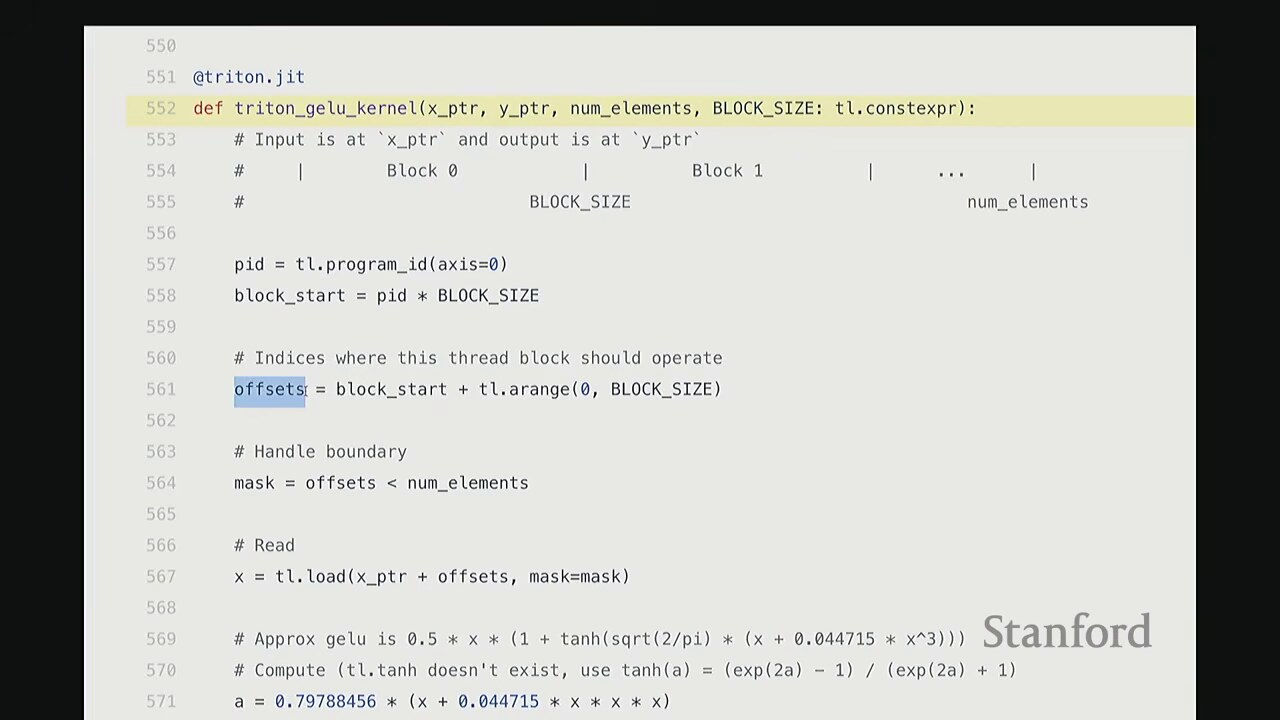
\includegraphics[width=\textwidth]{figures/fig_28_triton_gelu_code.jpg}
\caption{Triton GELU：\texttt{tl.arange} 生成块内偏移向量、\texttt{mask} 处理边界、\texttt{tl.load}/\texttt{tl.store} 向量化读写\protect\footnotemark}
\end{figure}
\footnotetext{视频画面时间区间：01:06:00--01:06:15。}

Triton 版 GELU 的 wrapper 与 CUDA 几乎一样：同样的 \texttt{assert}、\texttt{empty\_like}、grid 计算、\texttt{num\_blocks} 启动。关键差异在 kernel 本体——你不再算"单线程的下标 $i$"，而是算\textbf{一整块的偏移向量}：

\[
\text{offsets} = \text{pid} \times \text{BLOCK\_SIZE} + \text{tl.arange}(0, \text{BLOCK\_SIZE})
\]

\begin{itemize}
    \item \texttt{pid}（program id）相当于 CUDA 的 \texttt{blockIdx}，给出本 block 的起点。
    \item \texttt{tl.arange(0, BLOCK\_SIZE)} 生成一个长度为 \texttt{BLOCK\_SIZE} 的向量，代表块内所有线程的相对偏移——\textbf{注意这是一个向量，不是单个值}，因为你编程的是 block 不是 thread。
    \item \texttt{mask = offsets < n}：和 CUDA 的 \texttt{if (i < n)} 同理，但向量化——哪些位置越界由 mask 标出。
    \item \texttt{x = tl.load(x\_ptr + offsets, mask=mask)}：一次向量化加载整块数据到临时变量 $x$。
    \item 在 $x$ 上套 GELU 公式得到 $y$（同样是向量化运算）。
    \item \texttt{tl.store(y\_ptr + offsets, y, mask=mask)}：一次向量化写回。
\end{itemize}

整个心智模型从"我是一个线程"变成"我是一个 block，一次性处理一整块"，但代码结构其实和 CUDA 很像。

\subsection{PTX：贴近机器码的视角}

\begin{figure}[H]
\centering
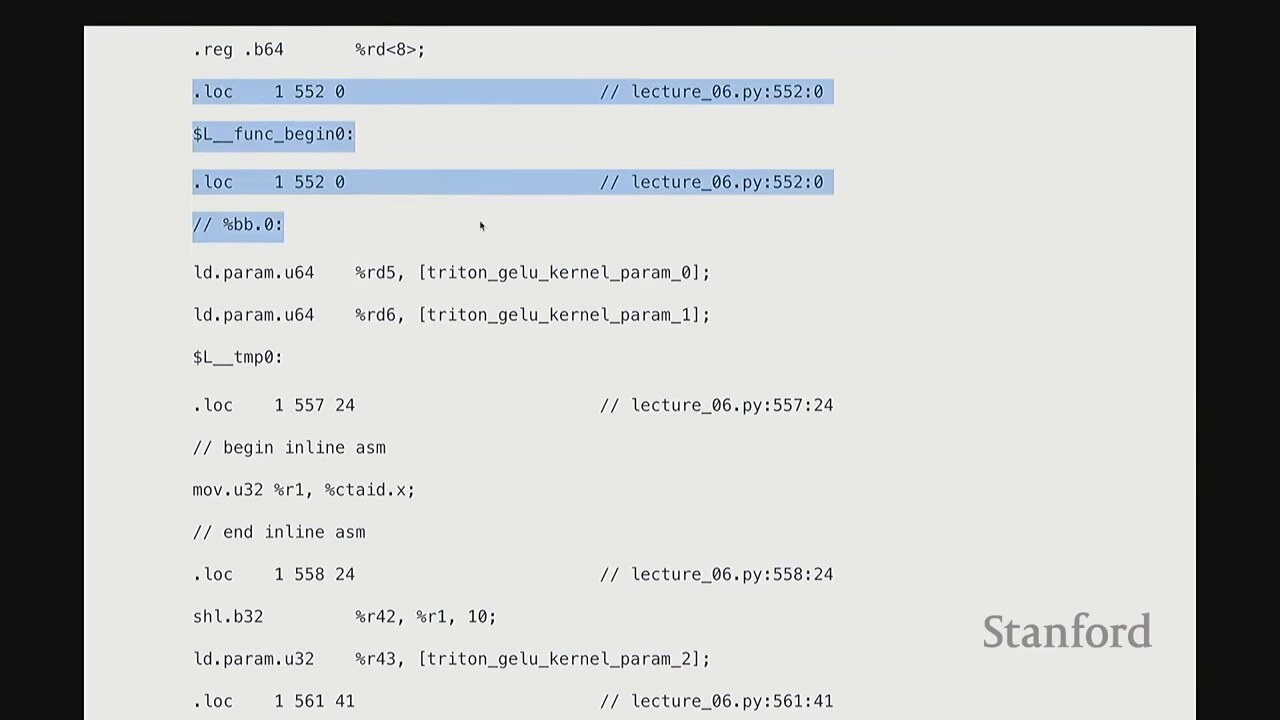
\includegraphics[width=\textwidth]{figures/fig_29_ptx_code.jpg}
\caption{Triton 编译出的 PTX：寄存器声明（\texttt{.b32}/\texttt{.f32}/\texttt{.b64}）、\texttt{ld.global} 四值合并加载、\texttt{mufu.tanh}、\texttt{st.global}\protect\footnotemark}
\end{figure}
\footnotetext{视频画面时间区间：01:09:00--01:09:15。}

Triton 最终会编译成接近机器码的 \textbf{PTX（Parallel Thread Execution）}代码。看 PTX 能直观感受 GPU 在线程级到底在干什么。合并加载的 4 值可以用一个简单的吞吐量关系刻画——单次 \texttt{ld.global.v4} 取回 4 个 float32，等效带宽为单次标量加载的 4 倍：

\[
\text{effective bandwidth} = 4 \times \text{(scalar load bandwidth)}
\]

\begin{itemize}
    \item 开头声明要用的\textbf{寄存器}：\texttt{.b32}（32 位无符号/字节级）、\texttt{.f32}（浮点计算用）、\texttt{.b64}（64 位，存指针）。
    \item 载入参数（x 指针、y 指针），算坐标偏移。
    \item \texttt{ld.global} 从 global memory 加载数据到寄存器：\texttt{ld.global.v4.b32 \{r2,r3,r4,r5\}, [rd1]}——注意\textbf{一次加载 4 个值}，这正是 Triton 自动 coalescing 的体现（硬件本来就免费送 4 个相邻值）。
    \item 一串浮点指令：乘常数、$x^3$（同数连乘）、用 \texttt{mufu}（math function unit）算 tanh、为把 $2^x$ 转成 $e^x$ 而乘 $\log 2$……逐步算出 GELU。
    \item 末尾 \texttt{st.global} 把结果寄存器（如 \texttt{r38--r41}）写回 \texttt{rd4} 指向的输出内存。
\end{itemize}

\begin{knowledgebox}{从 PTX 看到的两件事}
\begin{enumerate}
    \item 每个线程一次处理 \textbf{4 个值}（合并加载的体现）。
    \item 中间结果全部存在\textbf{寄存器}里——那是 GPU 上最快、最局部的存储。这就是为什么融合后的 kernel 快：数据不落 global memory。
\end{enumerate}
\end{knowledgebox}

\section{四种实现的总对比与 torch.compile}

\subsection{Triton 的性能}

\begin{figure}[H]
\centering
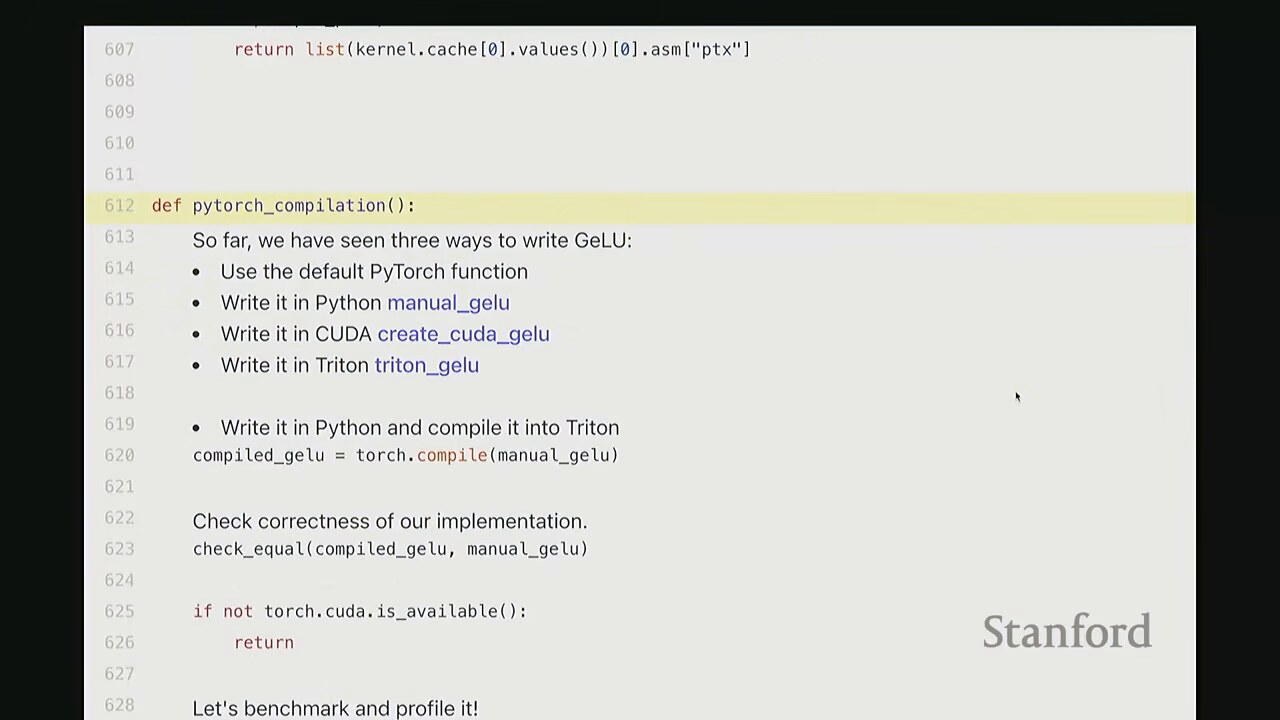
\includegraphics[width=\textwidth]{figures/fig_30_all_benchmarks.jpg}
\caption{GELU 四实现总对比：naive 8.1 / PyTorch 1.1 / CUDA 1.84 / Triton 1.848（毫秒）\protect\footnotemark}
\end{figure}
\footnotetext{视频画面时间区间：01:11:45--01:12:00。}

把四种实现摆在一起：naive 手写 \textbf{8.1 ms}、PyTorch \textbf{1.1 ms}、CUDA \textbf{1.84 ms}、Triton \textbf{1.848 ms}。Triton 没比 CUDA 更快，但\emph{写起来容易得多}——纯 Python、思考 block、向量化加法，复杂内存管理都交给编译器。profile 同样显示单 kernel 占满 GPU 时间。

\subsection{torch.compile：让 JIT 替你融合}

\begin{figure}[H]
\centering
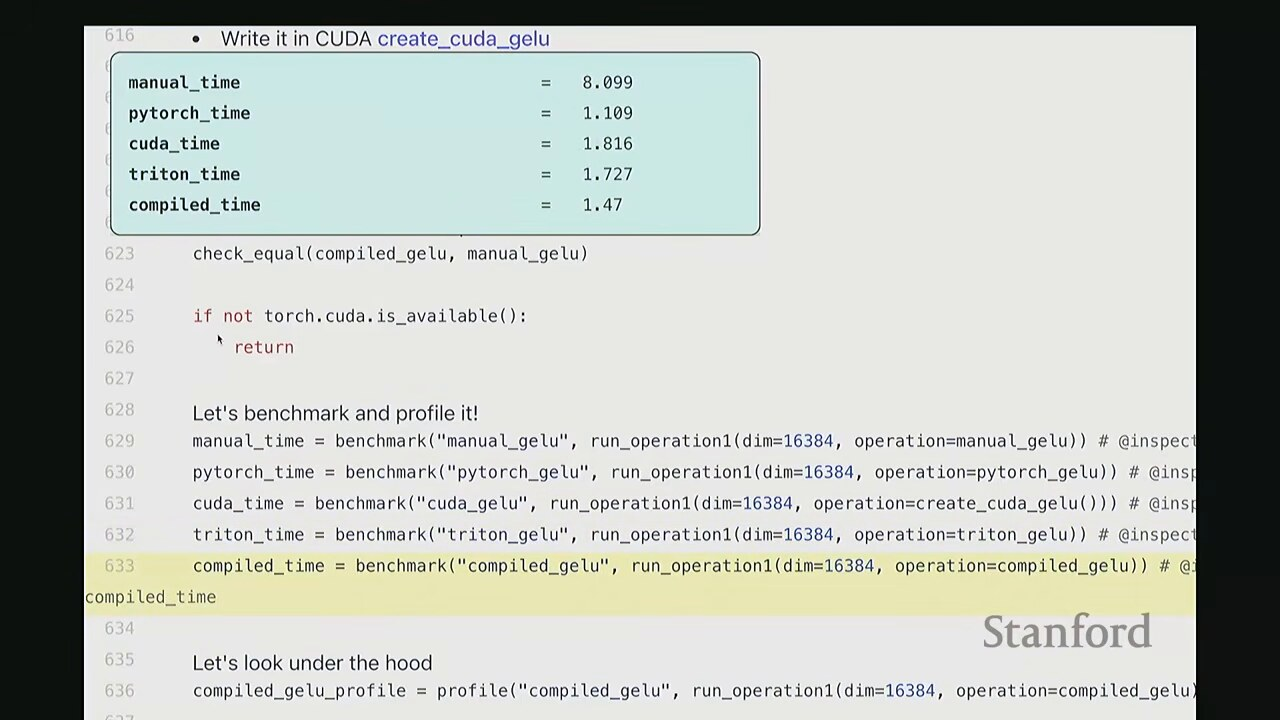
\includegraphics[width=\textwidth]{figures/fig_31_torch_compile.jpg}
\caption{\texttt{torch.compile}：JIT 自动做算子融合，底层生成 Triton，达到 1.47 ms\protect\footnotemark}
\end{figure}
\footnotetext{视频画面时间区间：01:12:45--01:13:00。}

写 CUDA kernel 很酷、很有成就感，但我们做的事其实很简单——把 $x^3$、exp、tanh 这些小运算塞进一个 kernel。\textbf{\texttt{torch.compile}} 能自动完成这件事：它接收未优化的 PyTorch 代码，自动尝试算子融合等优化，生成的"compiled GELU"在数值上等价。

\[
\text{naive 8.1 ms} \;>\; \text{CUDA 1.84 ms} \;\approx\; \text{Triton 1.848 ms} \;>\; \texttt{compile 1.47 ms} \;>\; \text{PyTorch 1.1 ms}
\]

\begin{importantbox}{现代 JIT 编译器相当强}
\texttt{torch.compile} 自动生成的代码（底层就是 Triton）甚至\emph{比我们手写的 Triton 还略快}（1.47 ms vs 1.848 ms）。结论是：对于简单的算子融合、matmul shape-specific 优化，JIT 已经做得很好，你不该轻易超过它。
\end{importantbox}

\subsection{什么时候仍要手写 kernel}

讲师被问到"什么时候你知道自己能比 torch.compile 做得更好"。回答是：

\begin{itemize}
    \item \textbf{简单的算子融合}：torch.compile 已经很强，你很难超过。
    \item \textbf{矩阵乘 shape-specific 优化}：torch.compile 知道形状后能挑最优 kernel，也很难超过。
    \item \textbf{非平凡的优化}：比如 \textbf{FlashAttention 1/2/3}——这些是相当非平凡的优化。如今 torch.compile 和 JAX 的 XLA 在\emph{ hindsight（事后）}知道该做哪些优化后，也能做；但 FlashAttention 3 还额外利用了 H100 的硬件级特性，这类东西 JIT 编译器\emph{很难自己发现}。
\end{itemize}

\begin{warningbox}{不要为了写 kernel 而写 kernel}
"你不该回家说'我要给语言模型的每个部分都手写 CUDA kernel'——那大概不是对时间的好的利用。"但如果你在写一个新架构、某块复杂逻辑跑不满利用率、而你又\emph{有理由相信}能做得更好——\textbf{那才是该掏出 Triton 的时候}。
\end{warningbox}

\begin{practicebox}{与 FlashAttention / Assignment 2 的关联}
Assignment 2 要求你写一个 \textbf{FlashAttention 2 的 Triton kernel}。FlashAttention 的核心是 \textbf{tiling（分块）+ online softmax（在线 softmax）}：把 $N^2$ 的注意力矩阵切成 tile，每个 tile 算完后立刻累积、不落盘完整的注意力矩阵，从而把注意力从 memory-bound 变成接近 compute-bound。这远比 GELU 复杂（需要 reduction、需要数值稳定的在线归一化），但本讲教的 Triton load/store/mask/block 编程模型正是它的基础。
\end{practicebox}

\section{Triton Softmax：一个需要 reduction 的例子}

\subsection{为什么 softmax 更难}

\begin{figure}[H]
\centering
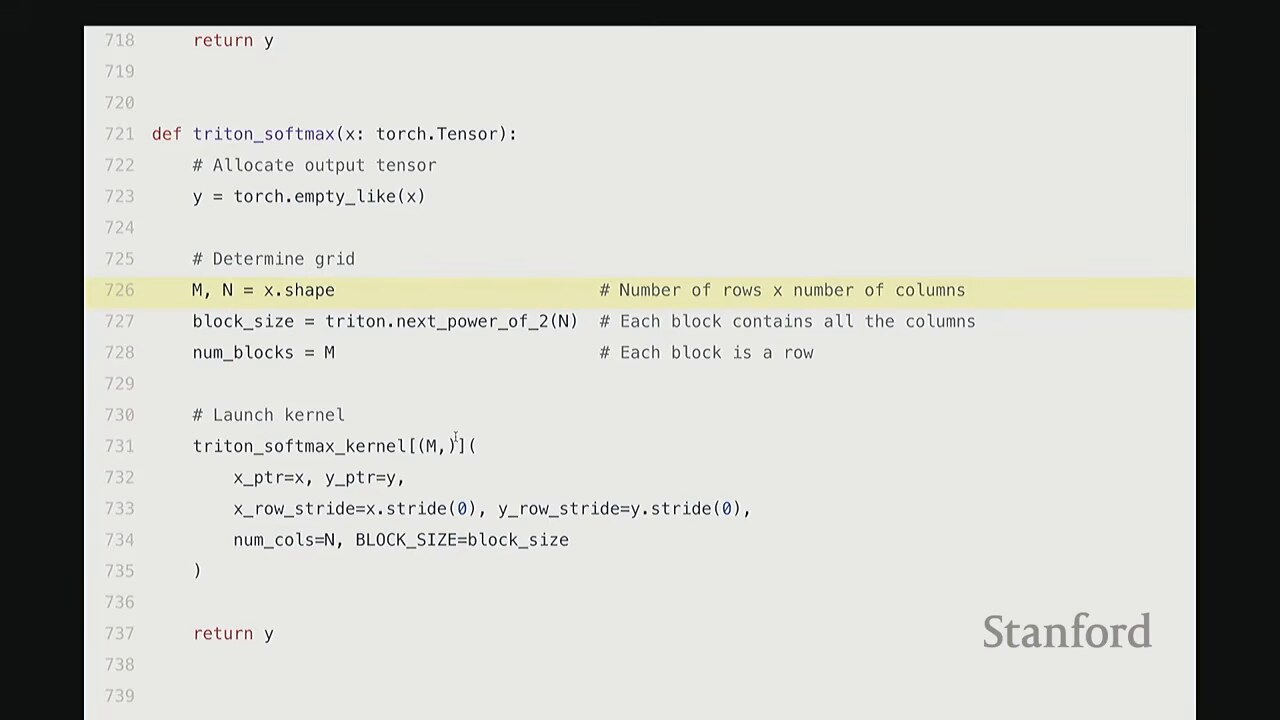
\includegraphics[width=\textwidth]{figures/fig_32_triton_softmax.jpg}
\caption{Triton softmax：一个 block 处理一行、\texttt{triton.next\_power\_of\_2} 把列数补到 2 的幂\protect\footnotemark}
\end{figure}
\footnotetext{视频画面时间区间：01:17:00--01:17:15。}

GELU 是纯 element-wise（每个元素独立），极好写。softmax 则有 \textbf{reduction}（要沿行求和），更接近真实场景。给定矩阵 $X \in \mathbb{R}^{R \times C}$，逐行做 softmax，朴素实现需要在每行上做两次全扫描（先 max 再 sum）。逐行计算开销为：

\[
\text{softmax}(X)_{i,j} = \frac{e^{X_{i,j} - \max_j X_{i,j}}}{\sum_k e^{X_{i,k} - \max_j X_{i,j}}}
\]

\begin{itemize}
    \item 先减去行最大值（数值稳定）。
    \item 取 exp。
    \item 沿行求和。
    \item 每个元素除以该和。
\end{itemize}

\subsection{一个 block 处理一行}

\textbf{关键设计}：让 grid 的每个 block 对应\emph{一行}。这样若一整行能塞进单个 SM 的 shared memory / 寄存器，求和就在 SM 内部完成，极快。具体做法：

\begin{itemize}
    \item \texttt{BLOCK\_SIZE = triton.next\_power\_of\_2(N\_COLS)}：把列数向上补到 2 的幂（便于向量化、便于 mask）。
    \item \texttt{num\_blocks = N\_ROWS}：每个 block 一行。
    \item kernel 内：算行索引、算列偏移、\texttt{tl.load} 整行进 SM、减 max、exp、求和、相除、\texttt{tl.store} 写回。
\end{itemize}

\begin{knowledgebox}{当计算能塞进一个 SM}
只要一行（或一个 tile）能整个装进 SM 的本地存储，写 Triton 就\emph{和写普通 Python 几乎一样}——只是多了 load/store 和 block 索引的记账。这就是 Triton 易用性的根源。
\end{knowledgebox}

\subsection{softmax 的性能对比}

\begin{figure}[H]
\centering
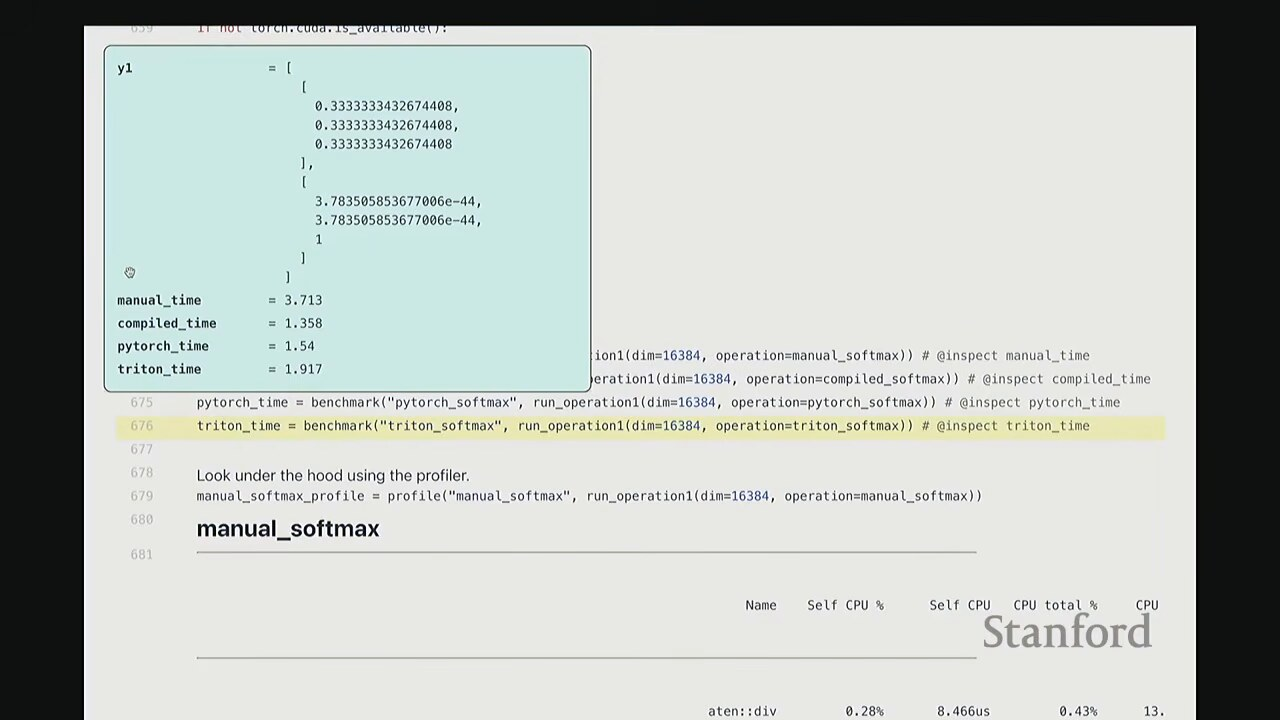
\includegraphics[width=\textwidth]{figures/fig_33_softmax_benchmark.jpg}
\caption{softmax 四实现对比：naive 3.7 / torch.compile 1.3 / PyTorch 1.5 / Triton 1.9（秒）\protect\footnotemark}
\end{figure}
\footnotetext{视频画面时间区间：01:19:00--01:19:15。}

softmax 的 benchmark：naive 手写 \textbf{3.7 秒}、\texttt{torch.compile} \textbf{1.3 秒}、PyTorch \textbf{1.5 秒}、Triton \textbf{1.9 秒}。这次 \texttt{torch.compile} 甚至\emph{超过了 PyTorch 官方实现}——因为它知道具体 shape 后能挑更优的融合方式。profile 里能看到：naive softmax 是一场灾难（到处都是 max、sum、exp 的零散 kernel 和反复的内存读写）；而 compile / PyTorch / Triton 都各自是一个融合好的单 kernel。

\section{总结与延伸}

\subsection{本讲核心要点}

\begin{knowledgebox}{五条可带走的经验}
\begin{enumerate}
    \item \textbf{永远先 benchmark 再 profile}：凭直觉猜瓶颈是浪费时间。理论只到 roofline，剩下全靠测量。
    \item \textbf{benchmark 三件套}：warm-up + \texttt{torch.cuda.synchronize()} + 多次取均值。少一个都会得到错误数字。
    \item \textbf{CPU/GPU 是异步解耦的}：CPU 提前把 kernel 排队，所以慢语言（Python）也能榨干 GPU；但任何"拉回 CPU"的操作（print、\texttt{.item()}）都会破坏流水线。
    \item \textbf{Kernel fusion 是性能钥匙}：把多个小算子融成一个，让中间结果留在寄存器，避免反复读写 global memory。
    \item \textbf{Triton 是 block 级的 Pythonic GPU 编程}：自动管 coalescing/shared memory，性能接近手写 CUDA，但开发体验好得多。
\end{enumerate}
\end{knowledgebox}

\begin{importantbox}{GELU 性能阶梯（全讲的一句话总结）}
\[
\underbrace{8.1\,\text{ms}}_{\text{naive 展开}} \;\to\; \underbrace{1.84\,\text{ms}}_{\text{手写 CUDA}} \;\to\; \underbrace{1.848\,\text{ms}}_{\text{Triton}} \;\to\; \underbrace{1.47\,\text{ms}}_{\texttt{torch.compile}} \;\to\; \underbrace{1.1\,\text{ms}}_{\text{PyTorch 官方}}
\]
融合一次就能拿到 4--8 倍加速，而 \texttt{torch.compile} 几乎"免费"就能拿到大部分收益。
\end{importantbox}

\subsection{动手建议与作业关联}

\begin{practicebox}{Assignment 2 里你会用到的东西}
\begin{itemize}
    \item \textbf{Nsight Systems}：profiling FlashAttention 2 实现，定位 memory-bound 瓶颈。
    \item \textbf{Triton}：亲手写 FlashAttention 2 kernel——tiling + online softmax，远比本讲的 GELU 复杂，但编程模型（load/store/mask/block）完全一致。
    \item \textbf{\texttt{torch.compile}}：作为 baseline 对比，看你的手写 kernel 到底比 JIT 强多少。
\end{itemize}
先 benchmark、再 profile、最后才动手写 kernel——这个顺序在作业里同样适用。
\end{practicebox}

\begin{warningbox}{不要忘记 CUDA\_LAUNCH\_BLOCKING}
写 CUDA/Triton kernel 出 bug 时，设 \texttt{CUDA\_LAUNCH\_BLOCKING=1} 让错误同步冒出来，否则堆栈对不上、几乎没法调试。这是讲师反复强调的"血泪经验"。
\end{warningbox}

\subsection{留待后续的问题}

本讲聚焦在\emph{单卡、单 kernel} 的高性能。但真实训练还涉及\textbf{并行}（数据并行、张量并行、流水线并行）——下一讲会讲 parallelism，那是 Assignment 2 的另一半。FlashAttention 的 tiling 与 online softmax 细节、KV cache 优化、推理时的 batching 等也留给后续。讲师结尾的鼓励："希望你们享受 Assignment 2。"

\end{document}
